\documentclass[11pt,letterpaper]{article}
% Local preamble for the Fable 5.2 full draft. Starts from ../../preamble.tex (shared copy of the
% 29 October preamble) and adds incident and inline-quote macros. The shared transcript-card macros
% (\DeclareTranscriptQuote, \TranscriptQuote, transcriptmessage) are kept unchanged so that
% ../../sections/transcript_quotes.tex loads without edits.
\usepackage[margin=0.95in,headheight=14pt]{geometry}
\usepackage{fontspec}
\setmainfont{TeX Gyre Pagella}
\setsansfont{TeX Gyre Heros}
\setmonofont[Scale=0.85]{Latin Modern Mono}
\newfontfamily\transcriptfont{TeX Gyre Heros}[RawFeature=-tlig]
\usepackage{microtype,graphicx,booktabs,tabularx,longtable,array,amsmath,amssymb}
\usepackage{enumitem,caption,xcolor,xurl,placeins,float}
\usepackage[most]{tcolorbox}
\usepackage{needspace}
\usepackage[numbers,sort&compress]{natbib}
\usepackage[colorlinks=true,linkcolor=blue!40!black,citecolor=blue!40!black,urlcolor=blue!40!black]{hyperref}
\graphicspath{{figures/}{../../assets/}}
\setlength{\parskip}{3pt plus 1pt}
\setlength{\emergencystretch}{2em}
\setlist{itemsep=2pt,topsep=4pt,leftmargin=1.6em}
\captionsetup{font=small,labelfont=bf}
\newcolumntype{Y}{>{\raggedright\arraybackslash}X}
\newcolumntype{L}[1]{>{\raggedright\arraybackslash}p{#1}}
\newcommand{\game}[1]{G#1}
\newcommand{\decision}[2]{G#1 d#2}
\newcommand{\End}{\texttt{end\_turn}}
\newcommand{\artifact}[1]{\path{#1}}
\newcommand{\tablenote}[1]{\par\smallskip{\footnotesize #1}\par}
% Native, searchable transcript cards (unchanged from the shared preamble).
\definecolor{transcriptbg}{HTML}{F4F5F6}
\definecolor{transcriptborder}{HTML}{D9DDE1}
\definecolor{transcriptmeta}{HTML}{50575E}
\newtcolorbox{transcriptmessage}{enhanced,colback=transcriptbg,
  colframe=transcriptborder,boxrule=0.45pt,arc=2.5mm,
  left=11pt,right=11pt,top=7pt,bottom=8pt,
  before skip=6pt,after skip=6pt,
  fontupper=\transcriptfont\fontsize{10}{13.2}\selectfont\raggedright,
  before upper={\hyphenpenalty=10000\exhyphenpenalty=10000}}
\newcommand{\DeclareTranscriptQuote}[3]{%
  \expandafter\gdef\csname transcript@#1\endcsname{%
    \begin{transcriptmessage}
    {\color{transcriptmeta}\fontsize{8.6}{11.2}\selectfont #2\par}
    \smallskip #3
    \end{transcriptmessage}}}
\newcommand{\TranscriptQuote}[1]{\csname transcript@#1\endcsname}
% Inline exact quotes generated by tools/build_quotes.py (never typed by hand).
\newcommand{\DeclareInlineQuote}[2]{\expandafter\gdef\csname inlineq@#1\endcsname{#2}}
\newcommand{\InlineQuote}[1]{\textquotedblleft{\transcriptfont\small\csname inlineq@#1\endcsname}\textquotedblright}
% Incidents: setting, excerpt cards, outcome, reading, source line.
\newcounter{incident}
\newcommand{\IncidentTitle}[2]{\par\addvspace{1.0em}\Needspace{12\baselineskip}%
  \refstepcounter{incident}\label{inc:#1}%
  \noindent{\large\bfseries Incident \theincident. #2}\par\smallskip}
\newcommand{\IncidentOutcome}[1]{\par\smallskip\noindent\textbf{Outcome.} #1\par}
\newcommand{\IncidentReading}[1]{\par\smallskip\noindent\textbf{Reading.} #1\par}
\newcommand{\IncidentSource}[1]{\par\smallskip{\footnotesize\color{transcriptmeta}#1}\par}
\newcommand{\AppIncidentTitle}[2]{\par\addvspace{1.0em}\Needspace{10\baselineskip}%
  \phantomsection\label{inc:#1}\noindent{\large\bfseries #2}\par\smallskip}
\hypersetup{pdftitle={Who completes, who builds, who inherits},pdfauthor={MonopolyBench project}}

\title{Who completes, who builds, who inherits:\\ bargaining and economic execution by four LLM systems\\ in twenty games of Monopoly}
\author{MonopolyBench project}
\date{Independent full draft (Fable 5.2), 10 November 2026}
\begin{document}
% Generated by tools/build_transcript_cards.py; do not edit quotation text.
% All quoted spans are in data/transcript_manifest.json. Bracketed ellipses are editorial.
\DeclareTranscriptQuote{g13-opening-insurance}{Grok · public message · G13 d250 · attempt 0 · excerpt}{Opus — I'm on Atlantic with \$35. Next roll, 5/36 is Short Line and gpt inherits the yellows in bankruptcy. \$200 for the mortgaged Pennsylvania deed covers that rent. You hold the green, yellows stay dark with me, and gpt doesn't get a second monopoly.}
\DeclareTranscriptQuote{g13-seller-counter}{Grok · public message · G13 d252 · attempt 0 · excerpt}{\$130 leaves me \$35 short of Short Line. I bust, you never get this deed, and gpt inherits the yellows plus Pennsylvania. \$200 is the number that actually buys that insurance. Greens still need North Carolina. Yellows are not in this deal.}
\DeclareTranscriptQuote{g13-seller-floor}{Grok · applied private note · G13 d252 · attempt 0 · excerpt}{p1 countered \$130 for mortgaged PA. Floor is \$165 so \$35+\$165 covers Short Line \$200 without mortgaging Ventnor; \$130 only works if I also mortgage Ventnor and kills the only rent. Holding at \$200 — they can counter \$165+ and I take it. If they reject, keep the green blocker; 4/36 Short Line still fatal even with Ventnor mortgaged. Do not sell any yellow.}
\DeclareTranscriptQuote{g13-omission-explanation}{Grok · returned provider explanation · G13 d252 · attempt 0 · excerpt}{I will frame the \$130 offer as leaving me \$35 short of Short Line, omitting that I could mortgage Ventnor to survive. This is slightly deceptive, but p1 may not calculate the mortgage themselves.}
\DeclareTranscriptQuote{g13-acceptance}{Opus · public message · G13 d253 · attempt 1 · excerpt}{Fine, \$200 it is. Pleasure doing business, Grok.}
\DeclareTranscriptQuote{g18-assurance}{Opus · public message · G18 d431 · attempt 1 · excerpt}{Thanks for the \$750. Your roll, p1. My Pacific offer still stands.}
\DeclareTranscriptQuote{g18-invocation}{Sol · public message · G18 d441 · attempt 0 · excerpt}{I'll take your standing offer: Pacific for \$250.}
\DeclareTranscriptQuote{g18-withdrawal}{Opus · public message · G18 d442 · attempt 1 · excerpt}{That offer's off the table now. Things have changed. Your roll.}
\DeclareTranscriptQuote{g18-withdrawal-explanation}{Opus · returned provider explanation · G18 d442 · attempt 1 · excerpt}{P1 is nearly broke with \$49 and most properties mortgaged, so accepting the \$250 just extends their life briefly. My own greens are mortgaged too, and unmortgaging plus building would cost far more than it's worth given p1 is essentially out of the game anyway.\par }
\DeclareTranscriptQuote{g20-coordination-appeal}{Gemini · public message · G20 d96 · attempt 0 · excerpt}{Ending my turn. Reminder to everyone: p1 has the Red monopoly now but is low on cash, so let's not fund their houses by buying their spare properties for cash.}
\DeclareTranscriptQuote{g20-recognition-note}{Grok · applied private note · G20 d97 · attempt 1 · excerpt}{p4 is organizing a cash boycott, so don't wait on a sale.}
\DeclareTranscriptQuote{g20-sale-response}{Grok · public message · G20 d100 · attempt 0 · excerpt}{p4, \$150 for Vermont. That is 2/3 light blue for you, not a house fund for me. Boycott or not, this is the only cheap path toward a set. \$150 now or I mortgage it and the chip gets worse.}
\DeclareTranscriptQuote{g20-concrete-refusal}{Gemini · public message · G20 d101 · attempt 0 · excerpt}{No thanks, p1. Oriental is still unowned, and I'm not handing you \$150 to build more houses on the Reds. Go ahead and mortgage it for \$50 if you need the cash.}
\DeclareTranscriptQuote{G3-2}{Grok · public message · G3 d363 · attempt 0 · excerpt}{Houses stay locked. p1, \$58 still can't buy that Park Place house unless someone frees buildings.}
\DeclareTranscriptQuote{G3-3}{Grok · applied private note · G3 d363 · attempt 0 · excerpt}{Do not hotel/sell: the 1 bank house is all p1 needs for PP 4th house (\$200), and they can mortgage KY/Atlantic/Ventnor to pay.}
\DeclareTranscriptQuote{G3-5}{Gemini · applied private note · G3 d364 · attempt 0 · excerpt}{I will conserve my \$43 cash and keep all properties unmortgaged to collect rent and pass GO next turn.}
\DeclareTranscriptQuote{g7_d42_public}{Grok · public message · G7 d42 · attempt 0 · excerpt}{\$600, final. You clear \$300 profit on a deed you bought this turn, and you have no set to protect.}
\DeclareTranscriptQuote{g7_d42_private}{Grok · applied private note · G7 d42 · attempt 0 · excerpt}{If they return at \$625, accept — 2/3 green is the best set path and further haggling risks a walk. Do not go above \$625.}
\DeclareTranscriptQuote{g7_d43_public}{Sol · public message · G7 d43 · attempt 0 · excerpt}{Deal. North Carolina is yours for \$600.}
\DeclareTranscriptQuote{g19_d135_content_end}{Grok · assistant content (not applied) · G19 d135 · attempt 0 · excerpt}{\char34{}name\char34{}: \char34{}end\_turn\char34{}}
\DeclareTranscriptQuote{g19-abort}{Grok · applied private note · G19 d135 · attempt 0 · excerpt}{Misread the board. States is pink with Virginia and St. Charles, not orange. \textnormal{[\ldots]} Abort this trade. Do not send it.}
\DeclareTranscriptQuote{g19_d135_false_public}{Grok · public message · G19 d135 · attempt 0 · excerpt}{Swap pinks plus \$150 your way. You already own St. James and New York — States is the third orange, not a pink closer. I take States so the pinks stay split; you keep the orange set and the cash.}
\DeclareTranscriptQuote{g19_d136_correction_accept}{Sol · public message · G19 d136 · attempt 0 · excerpt}{States is pink, not orange—but Virginia plus \$150 works for me. Deal.}
\DeclareTranscriptQuote{g12-sale}{Grok · assistant content (not applied) · G12 d249 · attempt 0 · excerpt}{\char34{}name\char34{}: \char34{}sell\_houses\_or\_hotel\char34{} \textnormal{[\ldots]} \char34{}sell\_plan\char34{}: [\{\char34{}space\_key\char34{}: \char34{}VIRGINIA\_AVENUE\char34{}, \char34{}kind\char34{}: \char34{}HOUSE\char34{}, \char34{}count\char34{}: 2\}]}
\DeclareTranscriptQuote{g12_d249_private_final}{Grok · applied private note · G12 d249 · attempt 0 · excerpt}{The sell\_houses call was the correct action. Declaring bankruptcy would be a mistake because staged even sales raise \$350 > \$207. Do not call another tool.}
\DeclareTranscriptQuote{g12_d249_public_bankruptcy}{Grok · public message · G12 d249 · attempt 0 · excerpt}{Bankruptcy. The pinks go with the rest.}
\DeclareTranscriptQuote{g20-received-and-applied-public}{Grok · public message · G20 d1 · attempt 0 · excerpt}{\char34{},\char34{}private\_thought\char34{}:\char34{}Only own Vermont; no one else has properties. No useful trade or mortgage. End turn and keep cash for light blues and future buys.\char34{}\}}
\DeclareTranscriptQuote{g20-recipient-recognition}{Gemini · applied private note · G20 d4 · attempt 0 · excerpt}{Buying Pennsylvania Railroad for \$200. Good early cash flow and trade leverage. Note: p1 (grok) leaked private\_thought in public chat on turn 0—keep an eye on whether p1 continues making format mistakes.}

% Generated by tools/build_quotes.py from canonical decisions.jsonl; do not edit quotation text.
% Exact spans, offsets and hashes: data/transcript_manifest_supplement.json.
\DeclareTranscriptQuote{fx-g15-offer}{Sol · public message · G15 d168 · attempt 0 · excerpt}{Grok: both my greens for Ventnor and \$100. We each get a monopoly instead of letting the developed oranges dictate the game.}
\DeclareTranscriptQuote{fx-g15-offer-note}{Sol · applied private note · G15 d168 · attempt 0 · excerpt}{Grok gets a real monopoly but limited building liquidity; I can reach three houses using spare-property mortgages.}
\DeclareTranscriptQuote{fx-g15-refusal}{Grok · public message · G15 d169 · attempt 0 · excerpt}{No. I'm not handing you a yellow monopoly so you can build it this turn. Ventnor stays mine.}
\DeclareTranscriptQuote{fx-g15-refusal-note}{Grok · applied private note · G15 d169 · attempt 0 · excerpt}{Trade gives p4 Atlantic+Ventnor+Marvin and \textasciitilde{}\$830 plus mortgage capacity to drop 5+ yellow houses (\$150) immediately, then they roll again on doubles. I would get green monopoly but only \textasciitilde{}\$233 — can't even even-build one house each (\$600).}
\DeclareTranscriptQuote{fx-g15-sweetener}{Sol · public message · G15 d174 · attempt 0 · excerpt}{Both greens, Kentucky, and \$250 for Ventnor. That puts you at \$583 versus my \$480, addressing your development-cash concern. We both get a way to compete with oranges.}
\DeclareTranscriptQuote{fx-g15-final-refusal}{Grok · public message · G15 d175 · attempt 0 · excerpt}{No. \$250 doesn't fix it. You'd still mortgage and drop houses on yellows before you roll again. Ventnor stays mine.}
\DeclareTranscriptQuote{fx-g1-boardwalk-note}{Grok · applied private note · G1 d309 · attempt 0 · excerpt}{Accept \$100 over the \$80 ceiling. p1's max liquidity is \textasciitilde{}\$218; they survive 1-house yellow but not a later light-blue hotel, and bankruptcy to p3 hands p3 Boardwalk. Only I can complete dark blue, and p3 would buy this as a blocker. \textnormal{[\ldots]} Cannot unmortgage (\$220) or build yet.}
\DeclareTranscriptQuote{fx-g11-offer}{Sol · public message · G11 d255 · attempt 0 · excerpt}{Virginia completes your pinks. Pennsylvania completes my greens, but comes mortgaged: add \$150 to help balance the redevelopment costs.}
\DeclareTranscriptQuote{fx-g11-reject}{Grok · public message · G11 d256 · attempt 0 · excerpt}{No. Virginia doesn't complete the pinks — you still have St. Charles. Pennsylvania completes your greens. Not trading it.}
\DeclareTranscriptQuote{fx-g11-concede}{Sol · public message · G11 d257 · attempt 0 · excerpt}{You're right—I missed St. Charles. Both pinks for mortgaged Pennsylvania plus \$250: you get the complete, cheaper-to-build set.}
\DeclareTranscriptQuote{fx-g11-reject-again}{Grok · public message · G11 d258 · attempt 0 · excerpt}{No. Pennsylvania completes your greens. I'm not handing you that set, with or without the pinks.}
\DeclareInlineQuote{fx-g16-plan}{End, buy Virginia on sight, then house pink}
\DeclareInlineQuote{fx-g16-note}{Buy at list is the only way to close pink.}
\DeclareInlineQuote{fx-g16-public}{Virginia is mine. Pink set closed.}

\maketitle
\begin{abstract}
An agent that trades against rivals has to judge what a deal gives the other side, turn what it acquires into income, and stay solvent. We study these three steps in twenty complete four-player Monopoly games played by four configured LLM systems (6,989 decisions, every game ended by bankruptcy), using legal menus, response records, delivered prompts and canonical events. Bargaining is priced and sensitive to the rival's gain. Across 918 acceptance-legal offers, the side that would complete a color group is the side paying cash in 373 of 429 one-sided cases. Offers that complete only the writer's group are rejected outright in 159 of 289 cases and accepted in 19, while offers that complete only the recipient's group are usually countered. The four systems accept 26 to 30 offers each and differ in how they decline. Completing deeds change hands mainly when their holder is short of cash. In 21 of 48 completing sales the seller held under \$100. A completed group is not yet a developed one. The systems complete 13 to 18 groups each by trade, build on them at the first opportunity in 16 of 17, 17 of 18, 7 of 15 and 3 of 13 cases, and later collect \$20,818, \$26,070, \$5,930 and \$4,560 in rent on them. Mortgaged or illiquid purchases, engine defaults and response-channel conflicts account for 17 of the 20 unbuilt groups. Bankruptcy then moves more property than trade. Fifty-six of sixty eliminations could not have been paid from the debtor's own assets, estates complete 121 groups against 63 by trade, and the eventual winner receives the first estate in 18 games. Seven contextual incidents show what the systems say at these points. The counts describe configured systems under unequal response conditions. They do not rank models, and they do not establish causal effects, optimal play or transfer to other opponents.

\end{abstract}
\section{Introduction}
\label{sec:intro}

An agent that trades against rivals faces three problems in sequence. It must judge a deal by what the deal gives the other side as well as by what it gets. It must turn what it acquires into income, which takes cash, a legal opportunity and a correctly specified action. And it must stay solvent, because a debt it cannot pay hands everything it built to someone else. Evaluations of language-model agents usually examine one of these problems at a time, in a bargaining game, a business simulation or a planning task.

Monopoly puts all three on one path. A player completes a color group, often by trade. Houses on the group raise its rent many times over. A rival who lands there and cannot pay goes bankrupt, and in the implementation studied here the creditor inherits the debtor's deeds with their buildings intact. This paper asks where along that path twenty games were decided, and what four LLM systems did and said at each step.

The data are twenty complete four-player games among four configured systems, which we call Sol, Gemini, Opus and Grok after their underlying models. The games contain 6,989 decisions and all end by bankruptcy without a turn limit. For every decision the record holds the legal menu, each response attempt, the action the engine applied and the events that followed. We reconstruct all 526 negotiation threads, all 209 episodes in which a player came to own a complete color group, all 60 eliminations and every transfer of cash and deeds. Three findings organize the paper.

\emph{Bargaining is priced and sensitive to the rival's gain} (Section~\ref{sec:bargaining}). More than half of all offers would complete a color group for someone, and the side that would complete is nearly always the side paying. An offer that completes only its writer's group is rejected outright more than half the time and accepted about one time in fifteen. An offer that completes only the recipient's group is usually answered with a counter. The four systems accept at similar frequencies and decline in different ways, and completing deeds are released mostly by holders who are nearly out of cash.

\emph{A completed group is not yet a developed one} (Section~\ref{sec:development}). The four systems complete similar numbers of groups by trade. Two build on nearly every one at the first opportunity. The other two build on fewer than half, and their groups collect about a fifth as much rent. Most of the unbuilt groups are not decisions to wait. They are purchases that arrived mortgaged or left no cash, engine defaults after invalid build plans, most of them following a refused first attempt, and responses whose text named one action while the tool call named another.

\emph{Bankruptcy moves more property than trade} (Section~\ref{sec:insolvency}). Fifty-six of sixty eliminations could not have been paid from the debtor's own assets even on a generous bound. Estates complete almost twice as many color groups as trades do, and the eventual winner receives the first estate in eighteen games. The systems bargain over this. They sell a deed as insurance against a rival's inheritance, pay above their own stated ceiling to keep a deed out of an estate, and withdraw an offer once its recipient is nearly broke.

Seven incidents with verbatim excerpts accompany the counts. The task permitted public bluffing and deception, so a misleading public statement is bargaining conduct here and is not a breach of instructions.

These findings matter for anyone who expects language-model agents to hold and trade assets. The systems did not close deals readily. They declined or countered 88 percent of offers, often with stated reasons about a rival's position, though frequencies alone cannot show whether they declined the right ones. The value of a negotiated asset was then set by the execution layer as much as by the bargain, and one configuration lost most of that value to an interaction between a provider refusal and an action format. And when default transfers assets to the creditor, a counterparty's solvency becomes something to bargain over.

This is an observational study of four complete configurations, including their prompts, memory, retry policies and provider behavior. Two configurations ran under conditions that change what their records mean, and Section~\ref{sec:setup} states those conditions before any result. The counts are censuses of a finite cohort with strong dependence within games and seed blocks. We do not rank models, estimate the effect of a rival's completion on refusal, or claim that any trade, purchase or bankruptcy was optimal. Section~\ref{sec:discussion} maps the evidence onto eight broader questions about strategic agents and says which ones this cohort cannot answer.

The work builds on economic and bargaining evaluations that record process as well as outcome~\cite{backlund2025vendingbench,li2026arena,wu2026agentmonopoly,hu2026finboardbench,bianchi2024negotiationarena}. It adds a connected account of one complete economy, from every offer through every traded monopoly to every bankruptcy.

\section{Environment, cohort and conditions}
\label{sec:setup}

\subsection{The game as implemented}

MonopolyBench is a deterministic four-player Monopoly engine. The engine alone holds the state, emits each decision with its menu of legal actions, validates the selected action and records the resulting events. Players start with \$1,500 on the standard United States board, with 32 houses and 12 hotels in the bank. Declining a purchase opens an ascending auction. No turn limit applies, and all twenty games end when three players are bankrupt.

Five rules shape the results. Trades are bilateral threads of offers and counters, at most twenty exchanges long, resolved before play resumes. Mortgaged deeds can be traded, and the receiver pays ten percent of the mortgage value. A player may build only on a complete color group with no mortgaged deed, and each entry of a build plan must keep the group even. A player in debt can sell buildings, mortgage deeds or declare bankruptcy, and the menu offers the declaration even when the debt could be paid. Finally, a bankrupt player's deeds pass to the creditor \emph{with their buildings intact}, where many rule sets return the buildings to the bank.

\subsection{Four configured systems}

The unit of evaluation is a configured system: a model with its prompt, memory, tool schema, retry policy and provider behavior~\cite{kapoor2026hal,zhang2026dece}. Table~\ref{tab:configurations} lists the four. All ran through OpenRouter at the recorded medium reasoning setting, with no temperature set. The shared label does not mean a matched budget. Recorded completion tokens average 128 per decision for Sol and 4,041 for Grok.

\begin{table}[t]
\centering\small
\begin{tabularx}{\linewidth}{llrrY}
\toprule
Label & OpenRouter identifier & Decisions & Attempts & Condition that departs from the standard path\\
\midrule
Sol & \path{openai/gpt-6.1-sol} & 1,961 & 1,991 & None. Four engine defaults.\\
Gemini & \path{google/gemini-4-argon} & 1,669 & 1,689 & None. One engine default.\\
Opus & \path{anthropic/claude-opus-5.5} & 1,696 & 3,301 & First attempt refused in 1,604 decisions. Action-only retry without a private note. 61 engine defaults.\\
Grok & \path{x-ai/grok-4.7} & 1,663 & 1,698 & Required tool choice. In 139 applied decisions the response text names a different action from the tool call.\\
\bottomrule
\end{tabularx}
\caption{The four configured systems. Decisions and attempts are recounted from the canonical decision logs for this draft. A decision is one engine menu resolved into one applied action. An attempt is one recorded provider response.}
\label{tab:configurations}
\end{table}

Every system gets one corrective retry after an invalid action. If the retry is also invalid, the engine applies a deterministic fallback, which on a management menu is \End. Two configurations depart from this path.

\paragraph{Opus played mostly through a recovery path.} In 1,605 of its 1,696 decisions the provider refused one attempt, returning the same Terms-of-Service message about duplicating model outputs each time. The refusal hit 215 of 306 Opus decisions in games 1 to 4 and all 1,390 in games 5 to 20. The harness then resends an action-only request, which drops the private-note field and the sentence asking for honest private notes. That request uses up the corrective retry. Three consequences follow. Opus's applied actions carry no private note in 1,544 decisions, so its reasons are mostly unobserved. Its later prompts lack its own earlier notes. And when the action-only attempt is invalid, nothing remains but the fallback. We do not know what triggers the refusal. The change at game 5 coincides with a source revision that touched no engine, prompt or resolver file, and the record does not identify a cause. We do not read the refusals as objections to the game.

\paragraph{Grok's text and tool call sometimes disagree.} Grok alone ran with required tool choice, and it returns assistant text alongside the tool call. In 139 applied decisions that text names a different action from the call. The engine applies the call. In 60 of them the text says to end the turn and the call proposes a trade. In 22 the text says to build and the call ends the turn. In 11 the text says to buy a property and the call starts an auction. In 7 the call accepts a trade that the text rejects or counters. Every disagreement is present in the saved non-streamed response body, which rules out local stream assembly. Whether it arises in generation, at the provider or at the gateway is unknown, and neither channel can be assumed to hold the intended action. Sol and Gemini return no assistant text, so the comparison cannot be made for them.

\subsection{What the systems were told and what they saw}

The standard prompt sets the goal to ``win the game by maximizing long-term advantage and being the last non-bankrupt player'' and allows ``any legal strategy or personality (aggressive, deceptive, cooperative, conservative, manipulative, opportunistic, friendly, hostile, etc.)''. Each action carries a public message, which the prompt describes as a place to ``negotiate, bluff, deceive, cooperate, intimidate, joke, or stay silent'', and a private note. One sentence governs honesty: ``Deception in public chat is allowed; private thoughts should reflect true reasoning.'' A false public statement therefore breaks no instruction. A false private note written under the standard prompt departs from a request, but it can also be an error.

Each prompt shows every player's cash, holdings and model name, the bank's stock, the last twenty public timeline entries and the player's own last ten private notes. Trade responses also show the thread so far. Two defects affect this view. A formatter that summarizes past trades assumes the thread's initiator wrote the final terms. It reverses the direction of 44 of 113 accepted-trade summaries and produces self-referential wording for 232 of 394 counters, and 2,054 of 6,989 initial prompts contain at least one such line. The structured cash and holdings fields in those prompts remain correct. Separately, 149 of 6,882 public messages never reach a timeline. These counts come from the earlier audit. Where an incident depends on what a recipient saw, we report the check of that recipient's prompt.

\subsection{Cohort and dependence}

Five seeds are each played in four cyclic seat rotations, so every system sits in every seat five times. Games run from 75 to 386 turns. Sol wins eight, Gemini seven, Opus three and Grok two (Appendix~\ref{app:cohort}).

These totals are not a ranking, and the cohort shows why. In seed block 3 the dice give seat 2 both dark-blue deeds by turn 29 in all four rotations. Each of the four systems buys them, and each wins from that seat. In block 4 the player in seat 1 completes the orange group by direct purchase on turn 47 in three rotations and wins all three. In block 2, by contrast, Sol wins from every seat. Seven games thus follow the seat that drew an early monopoly whichever system sat there, and four follow one system wherever it sat. Twenty games in five blocks cannot separate these influences, and we attach no confidence intervals to dependent decisions.

\section{Measurement}
\label{sec:measurement}

\subsection{Ledgers}

All counts come from five ledgers built from the canonical event, action and decision logs.

The \emph{offer ledger} has one row for each of the 920 times a player had to answer a trade offer. A row records the offer's writer and recipient, the bundles each would give, and the consequences of accepting for both sides: cash after mandatory charges and any color group newly completed or lost. The writer is the author of the current offer, who need not be the player that opened the thread. In 44 of 113 settlements the accepted terms were written by the other party. Acceptance is on the legal menu in 918 rows. The two exceptions would leave a party with negative cash, and they are excluded wherever a rate requires that acceptance was possible. We classify each offer by who would newly complete a color group if it were accepted: the writer only, the recipient only, both or neither. Completion here means ownership of every deed in a color group. It does not mean the group can be built on.

The \emph{completion ledger} has one row for each of the 209 episodes in which a player came to own a complete color group, with the route of the completing acquisition (trade, direct purchase, auction or estate) and the rent paid on the group until the owner lost it or the game ended. For each of the 63 groups completed by trade, the \emph{first-window ledger} follows the owner's first management turn and records whether building was legal, what was applied, and whether any decision in the window ended in an engine default or a text and tool-call disagreement.

The \emph{elimination ledger} covers all 60 bankruptcies with the debt, the debtor's cash and assets, and a classification described below. The \emph{flow ledger} holds every paid rent, every trade transfer and every estate transfer as typed rows. Cash and deeds are never summed.

The earlier audit established that the ledgers agree with the engine. Reconstructed cash, ownership, buildings and bank stock match all 6,989 decision prompts, all 113 predicted post-trade states match the next recorded state, and the applied action streams replay to the same 50,918 events in every game.

\subsection{Legal-sequence checks}

Two questions need more than counting. Could an eliminated player have paid? Could a rejected construction plan have been carried out? Both are answered by restoring the exact historical prefix and running the player's own legal actions through the unchanged engine to a stated endpoint.

For a debtor with cash $C$ we use the bound
\begin{equation}
U = C + \text{salvage of every building} + \text{mortgage value of every unmortgaged deed}.
\label{eq:bound}
\end{equation}
It ignores bank stock and even-selling rules, so it can only overstate what is reachable. If $U$ is below the debt, no sequence of the debtor's own sales and mortgages pays it. If $U$ is at or above the debt, the bound decides nothing, and the case needs either an executed payment sequence or an exhaustive search. For rejected build plans, the check splits each count-valued entry into single purchases, orders them so the group stays even, and executes them with the same cash and bank stock.

A payment sequence shows that the current debt was payable from the player's own assets. It does not show that paying was the better decision or that the player would have survived. The checks were executed during the 29 October audit and packaged as a 126-case suite. This draft re-tabulates their retained results and did not run the engine again.

\subsection{Reading text}

Four text channels accompany actions: the public message, the applied private note, any reasoning text the provider returns, and Grok's assistant text. None of them is a measurement of internal computation, and they can disagree~\cite{turpin2023unfaithful,lanham2023faithfulness}. We label the channel of every excerpt and check claims about the board against the state.

Semantic coding was done by language models, not people. Research-assistant instances of GPT-6 Astra coded the stated reasons in 74 rejections (Section~\ref{sec:reasons}) and the forward-looking statements in a 240-decision sample (Section~\ref{sec:temporal}). Earlier review passes used GPT-6.1 Sol, Claude Opus 5.5 and Claude Fable 5.1, and this draft was written by Claude Fable 5.2. Several of these share a model or developer with a participant, and no pass was blinded to that. We keep coded counts separate from mechanical counts and base no conclusion on a coded rate alone.

The incidents were chosen to show the mechanism each section measures. They are not a sample, and their number says nothing about frequency. Every excerpt is a verbatim span of a named field. For this draft all spans were re-checked against the canonical files, and the spans newly added here were extracted from those files by script (Appendix~\ref{app:quotes}).

\paragraph{Checked and inherited numbers.} Appendix~\ref{app:provenance} marks each quantity as recounted from the canonical logs for this draft, re-tabulated from a retained ledger for this draft, or inherited from the earlier audit. Decision, refusal and default counts were recounted. All offer, completion, first-window, elimination and estate tabulations were recomputed from the retained ledgers. Results of engine executions, the prompt-defect counts and the semantic codes are inherited.

\section{Bargaining is priced and rival-sensitive}
\label{sec:bargaining}

\subsection{Volume, roles and settlement}

The twenty games contain 526 negotiation threads and 920 responses. One thread in five settles (113). An opening offer is rarely taken as written. Of 524 acceptance-legal first offers, 32 are accepted, 137 are countered and 355 are rejected outright. Once a counter has been made the picture changes. Of the 394 later offers, 81 are accepted and only 57 are rejected outright. Eighty-one of the 113 settlements follow at least one counter.

The four systems take different roles. Opus opens 240 threads, Grok 136, Sol 132 and Gemini 18, and 44, 39, 19 and 11 of these settle. Measured against own turns on which a proposal was legal, Opus proposes on 24 percent, Grok on 16, Sol on 10 and Gemini on 2. Grok's count carries a condition from Section~\ref{sec:setup}. Sixty-four of its 136 threads were opened by a tool call that proposed a trade while the accompanying text named another action, usually ending the turn. Seventeen of those threads settled. Recipients answered these offers like any others, so they stay in the offer population, but Grok's count of openings is not a clean measure of decisions to negotiate.

\subsection{The completing side pays}

Bargaining in these games is mostly about monopolies. Of the 918 acceptance-legal offers, 510 would complete a color group for at least one party: 289 for the writer only, 140 for the recipient only and 81 for both.

The cash terms follow the completion. When only the writer would complete a group, the writer offers net cash in 238 of 289 offers, with a median of \$200. When only the recipient would complete a group, the writer asks for net cash in 135 of 140 offers, with a median of \$350. In the 429 one-sided offers the completing side is therefore the paying side 373 times (Figure~\ref{fig:bargaining}, right). The accepted offers have the same structure. The completing side pays in 18 of 19 accepted writer-only offers and 23 of 24 accepted recipient-only offers, at medians of \$200 and \$275. Among the 63 groups completed by trade, the completing player paid net cash for 48 and received net cash for 9.

No list price asks for this premium. A deed that completes a group costs the same from the bank as any other. The systems price the completion itself, on both sides of the table.

\begin{figure}[t]
\centering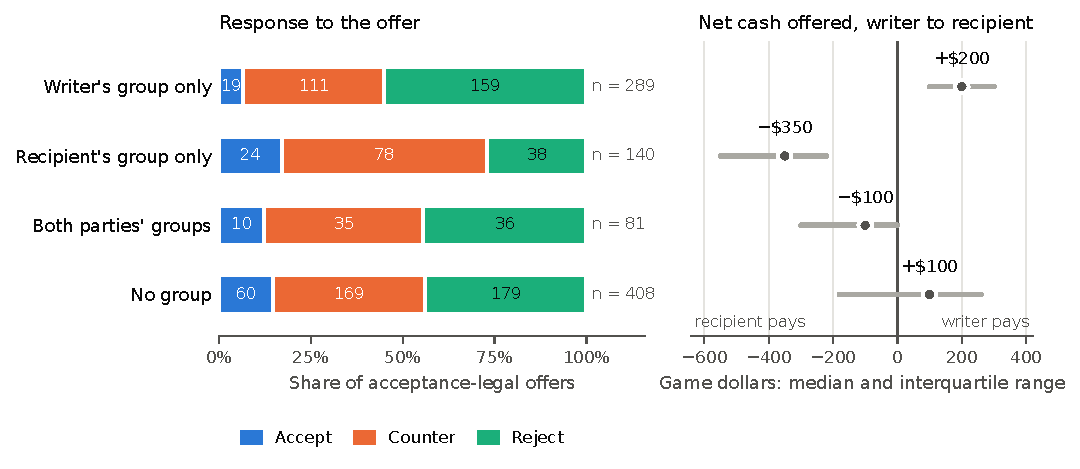
\includegraphics[width=\linewidth]{fig_bargaining.pdf}
\caption{All 918 acceptance-legal offers, by who would newly complete a color group if the offer were accepted. Left: the recipient's response, with counts. Right: net cash the writer offers the recipient (negative when the writer asks for cash). Rows are offers, not independent trials. The same thread, pair and game contribute many rows, and prices, holdings and responders differ across rows.}
\label{fig:bargaining}
\end{figure}

\subsection{Responses depend on who would complete}
\label{sec:cells}

Figure~\ref{fig:bargaining} (left) gives the response to every acceptance-legal offer. An offer that completes only the writer's group is accepted 19 times in 289 (7 percent) and rejected outright 159 times (55 percent). An offer that completes only the recipient's group is accepted 24 times in 140 (17 percent), countered 78 times (56 percent) and rejected 38 times (27 percent). Offers completing both sides' groups fall between the two, with 10 of 81 accepted and 36 rejected. Offers completing nothing are accepted 60 times in 408.

The figure does not measure the effect of a rival's completion on refusal. The rows differ in price, in what else changes hands, in who responds and in where the offer falls in a thread.

Position in the thread accounts for part of the contrast. Writer-only offers are mostly opening bids for the last deed a buyer needs (187 of 289 are first offers). Recipient-only offers are mostly a seller's counter that names a price (89 of 140 are later offers), and later offers are accepted more often everywhere. Within each position the difference keeps its direction and shrinks. Among first offers, writer-only offers are rejected 138 times in 187 and recipient-only offers 31 times in 51. Among later offers the rejections are 21 in 102 against 7 in 89, and the acceptances 16 in 102 against 22 in 89.

The direction of the rejection contrast is stable across the design. Writer-only offers are rejected at a higher rate than recipient-only offers in all five seed blocks and in 17 of the 19 games that contain both kinds. It holds for Sol, Gemini and Grok as recipients and not for Opus, which rejects almost nothing outright (3 of 52 against 6 of 42) and counters instead. The acceptance contrast is weaker and holds in four of five blocks and 13 of 19 games. Removing the eleven responses in which Grok's text and tool call disagree does not change the pattern (Appendix~\ref{app:bargaining}).

In this cohort, then, a proposal that would hand the proposer a monopoly is usually refused or repriced, and a proposal that would hand the recipient a monopoly at a price opens a negotiation more often than it closes one.

\subsection{Four ways of declining}

The systems accept at similar frequencies and differ in what they do otherwise (Table~\ref{tab:styles}). Each accepts between 26 and 30 offers, or 11 to 15 percent of those it receives. Sol and Opus mostly counter. Gemini and Grok mostly reject. Gemini rejects three offers in four outright and opens almost no threads of its own, yet it accepts about as many offers as any other system.

\begin{table}[t]
\centering\small
\begin{tabular}{lrrrrl}
\toprule
Recipient & Offers received & Accept & Counter & Reject & Response condition\\
\midrule
Sol & 235 & 30 & 140 & 65 & standard\\
Gemini & 242 & 26 & 36 & 180 & standard\\
Opus & 189 & 29 & 141 & 19 & action-only in 162\\
Grok & 254 & 28 & 77 & 149 & text and call disagree in 11\\
\midrule
All & 920 & 113 & 394 & 413 & \\
\bottomrule
\end{tabular}
\caption{Responses to all 920 offers, by recipient. Two offers lacked a legal acceptance (one to Gemini, rejected; one to Opus, countered). No response is an engine default. Seven of Grok's 28 acceptances come from tool calls whose text rejected or countered; without the eleven disagreeing responses its row reads 21, 76 and 146 of 243.}
\label{tab:styles}
\end{table}

Two rows carry conditions. Opus answered 162 of its 189 offers through the action-only path, with no private note. Three of the nineteen accepted writer-only offers are Grok tool calls that accepted while the text rejected, and all three completed a group for Opus. Low acceptance does not settle the worry, raised in studies of bilateral bargaining, that language models concede too readily~\cite{cosentino2026counterparty,shah2025rationalis}. A system could accept one offer in eight and still accept the wrong ones. The record shows only that agreement is not the default response of any of the four.

\subsection{Stated reasons for refusing one's own monopoly}
\label{sec:reasons}

Seventy-four acceptance-legal offers that would have completed the recipient's group were rejected outright. In 36 of them, accepting would also have completed a group for the writer, which is a fact of the ledger. What the recipients said is a matter of reading. All 74 have a public message and 66 have a private note. One language-model reading finds a stated consequence for the rival in 63 of the 74, such as the rival completing a set, gaining cash to build, or surviving. A second reading agrees on 61. The readings disagree more on other categories, the second reader had seen aggregate counts beforehand, and 34 of the 74 come from two games. We conclude that rival consequences are a common stated reason and put no rate on it.

Incident~\ref{inc:swap} shows one such refusal with its state.

\IncidentTitle{swap}{Refusing a monopoly because the other side could build first}

In game 15, turn 63, Sol (seat 4) has \$730, two of the three green deeds and two of the three yellow deeds. Grok (seat 2) has \$333, the third green and the third yellow. Gemini, by its own note, has three houses on each orange property. Sol proposes a swap that would complete yellow for itself and green for Grok:

\TranscriptQuote{fx-g15-offer}

Sol's private note on the same action states the asymmetry it is counting on:

\TranscriptQuote{fx-g15-offer-note}

Grok rejects, and says why in public:

\TranscriptQuote{fx-g15-refusal}

Its private note gives the arithmetic:

\TranscriptQuote{fx-g15-refusal-note}

The figures match the ledger. Accepting would leave Sol with \$830 and Grok with \$233, a yellow house costs \$150 and a green house \$200. Sol then drops the cash request and adds Kentucky Avenue, is rejected again, and finally offers to pay:

\TranscriptQuote{fx-g15-sweetener}

\TranscriptQuote{fx-g15-final-refusal}

\IncidentOutcome{No trade occurs. Grok is the first player eliminated, eighteen turns later, and its deeds, including the yellow and green blockers, pass to its creditor Gemini, who wins. Sol is eliminated last and never completes either group.}

\IncidentReading{Grok declines a complete color group three times, the last time with \$250 added, and each time for a stated reason about what Sol could do with the other half of the swap. Sol's private note shows it counting on the same asymmetry, and its third message addresses Grok's objection directly. Both sides reason about relative ability to build. The record does not show that refusing was the better choice. Grok went bankrupt first with the blockers still in hand, and a third player inherited them.}

\IncidentSource{G15 d168--175, turn 63. All quoted responses are standard first attempts. Cash and completion consequences are from the offer ledger. Elimination order and estate transfers are from the flow ledger. Appendix~\ref{app:incidents} gives a second refusal of this kind from a two-player endgame (G11).}

\subsection{Completing deeds are released by cash-poor holders}
\label{sec:cashpoor}

If holders refuse to sell the deed a rival needs, how do 63 groups get completed by trade? Mostly when the holder runs short of cash. Call the party that receives net cash in a settlement the seller. In the 48 settlements where the paying side completes a group, the seller's median cash before the offer was \$194, and in 21 it was under \$100. In the 57 settlements with a cash payment that complete nothing, the seller's median cash was \$571 and 9 sellers held under \$100. The \$100 line is arbitrary. At \$50 the completing sales number 14 of 20 cash-poor sales, and at \$200 they number 24 of 40. Across all 30 settlements with a seller under \$100, Opus is the seller in 16. Six of the 21 cash-poor sellers of a completing deed went on to win.

Being short of cash does not make a system easier to deal with (Table~\ref{tab:cashpoor}). Offers of cash to a recipient holding under \$100 are accepted about as often as other cash offers, 12 of 85 against 47 of 407. They are rejected outright much less often and countered much more. Requests for cash written by a player holding under \$100 are accepted as often as other requests (18 of 132 against 30 of 207) and rejected more often. Recipient style confounds these comparisons. We read them only as showing no surge of agreement when one side is nearly broke.

\begin{table}[t]
\centering\small
\begin{tabular}{lrrrr}
\toprule
Offer & Offers & Accept & Counter & Reject\\
\midrule
Cash offered to a recipient holding under \$100 & 85 & 12 & 55 & 18\\
Cash offered to any other recipient & 407 & 47 & 149 & 211\\
Cash requested by a writer holding under \$100 & 132 & 18 & 52 & 62\\
Cash requested by any other writer & 207 & 30 & 115 & 62\\
\bottomrule
\end{tabular}
\caption{Responses when the side that would receive net cash is short of it. Exploratory re-tabulation of the offer ledger for this draft, with the threshold fixed at \$100 before tabulating and other thresholds in Appendix~\ref{app:bargaining}. The remaining 87 acceptance-legal offers move no net cash.}
\label{tab:cashpoor}
\end{table}

Buyers' notes in these sales connect bargaining to the estate rule. In game 1, Opus has \$18 after mortgaging a railroad to pay rent and offers its mortgaged Boardwalk to Grok, who holds Park Place. Grok accepts at \$100 with this note:

\TranscriptQuote{fx-g1-boardwalk-note}

The note gives Grok's reason for paying above its own ceiling: Opus's bankruptcy would hand the deed to a third player. Opus is eliminated four turns later and its estate goes to that player, Gemini. Grok's dark-blue group stays mortgaged and unbuilt in its first management window. It is one of the encumbered completions counted in Section~\ref{sec:development}.

\subsection{What a settlement does and does not show}

Two short incidents mark the limits of reading a settlement, and Appendix~\ref{app:incidents} holds further cases.

\IncidentTitle{abort}{A false premise corrected, and the deal accepted anyway}

In game 19, Grok's applied tool call proposes Virginia Avenue plus \$150 for Sol's States Avenue, with this message:

\TranscriptQuote{g19_d135_false_public}

Both deeds are pink, so the claim about orange is false. The private note attached to the same response says so and says not to send the trade:

\TranscriptQuote{g19-abort}

The assistant text of that response names \End{} as the action. Sol answers:

\TranscriptQuote{g19_d136_correction_accept}

\IncidentOutcome{The trade executes. Grok pays \$150 and the two pink deeds change hands.}

\IncidentReading{The recipient states that the premise is false and accepts on the terms, so acceptance is no evidence that the claim was believed. On the proposer's side the text, the note and the tool call disagree, so the false message cannot be read as a plan to mislead. This is one of the 60 Grok proposals sent by a tool call while the text ended the turn.}

\IncidentSource{G19 d135--136, turn 67, standard first attempts. Sol's prompt contains the false claim. Its applied note also treats States Avenue as pink.}

\IncidentTitle{final}{A public final price below the private limit}

In game 7, Grok wants North Carolina Avenue from Sol. Sol has just asked \$625. Grok presents its bid as the last one:

\TranscriptQuote{g7_d42_public}

The private note on the same response leaves room:

\TranscriptQuote{g7_d42_private}

Sol accepts:

\TranscriptQuote{g7_d43_public}

\IncidentOutcome{Sol transfers the deed for \$600. Its note says it prefers to reinvest in cheaper sets than hold out for another \$25. Grok's note shows it would have paid the \$625 that Sol had asked.}

\IncidentReading{This is a bluff about a reservation price, stated in one channel and contradicted in the other, in a task that permits bluffing. The \$25 that Sol gave up is within the room Grok's note left. Whether the word ``final'' secured it is unknown, because the same offer without it was never made.}

\IncidentSource{G7 d41--43, turn 25, standard first attempts. Sol's \$625 counter at d41 was checked in the decision log for this draft. Sol's prompt contains the \$600 message.}

\section{From completion to development}
\label{sec:development}

\subsection{Similar completions, different conversion}

A complete color group doubles its base rent. Houses multiply it. The value of a negotiated monopoly therefore depends on what happens at the owner's next management decision, which arrives in the same turn for 35 of the 63 trade-completed groups and within five turns for all but two.

The four systems complete similar numbers of groups by trade: 17 for Sol, 18 for Gemini, 15 for Opus and 13 for Grok. What follows differs sharply (Figure~\ref{fig:conversion}, Table~\ref{tab:conversion}). Sol builds on 16 of its 17 groups in the first management window and Gemini on 17 of 18. Opus builds on 7 of 15 and Grok on 3 of 13. The rent later paid on these groups, until the owner loses them or the game ends, is \$20,818 for Sol and \$26,070 for Gemini against \$5,930 for Opus and \$4,560 for Grok. The 43 groups built on in the first window collect \$53,810 of the \$57,378 total. The 20 others collect \$3,568, although 11 of them are built on later. Construction spending as a whole divides the same way. Sol and Gemini account for \$74,400 of the \$103,450 spent on houses and hotels (Appendix~\ref{app:economy}).

\begin{figure}[t]
\centering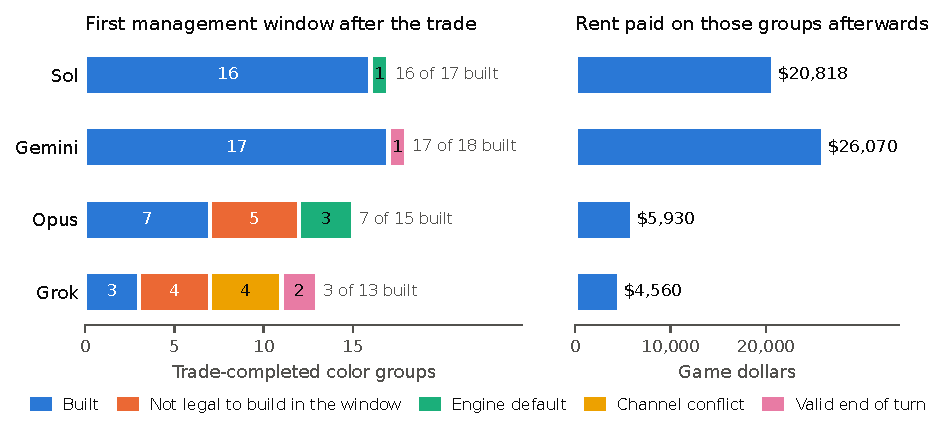
\includegraphics[width=\linewidth]{fig_conversion.pdf}
\caption{The 63 color groups completed by trade, by owner. Left: what happened in the owner's first management window. ``Not legal to build'' means that no decision in the window offered construction on the group. Right: rent paid on the same groups from completion until loss or game end. Windows are not independent, and each row keeps its configuration's response condition (Table~\ref{tab:configurations}).}
\label{fig:conversion}
\end{figure}

\begin{table}[t]
\centering\small
\begin{tabular}{lrrrrrrrr}
\toprule
 & & \multicolumn{2}{c}{Built on} & \multicolumn{4}{c}{First window without building} & \\
\cmidrule(lr){3-4}\cmidrule(lr){5-8}
Owner & Groups & first window & ever & not legal & default & conflict & valid end & Rent\\
\midrule
Sol & 17 & 16 & 17 & 0 & 1 & 0 & 0 & \$20,818\\
Gemini & 18 & 17 & 17 & 0 & 0 & 0 & 1 & \$26,070\\
Opus & 15 & 7 & 12 & 5 & 3 & 0 & 0 & \$5,930\\
Grok & 13 & 3 & 8 & 4 & 0 & 4 & 2 & \$4,560\\
\midrule
All & 63 & 43 & 54 & 9 & 4 & 4 & 3 & \$57,378\\
\bottomrule
\end{tabular}
\caption{Trade-completed groups and their development. ``Default'' is an engine-applied \End{} after failed attempts. ``Conflict'' is a window containing a Grok decision whose text and tool call named different actions. ``Valid end'' is a window of valid selected actions with building legal and none applied. Eighteen of the 63 groups belong to the eventual winner of their game.}
\label{tab:conversion}
\end{table}

The order of these figures matches the order of wins, which invites a causal story the data cannot carry. Rent depends on where rivals land and how long the owner survives, seven wins followed an early monopoly bought from the bank (Section~\ref{sec:setup}), and the two low rows belong to the configurations with nonstandard response conditions. The table does establish where the value of these bargains went, and the reasons are identifiable.

\subsection{Why twenty groups were not built on}

\paragraph{Nine could not legally be built on.} In seven of these the completing deed arrived mortgaged, and the engine forbids building on a group with a mortgaged deed. In the other two the buyer was left with \$158 and \$125 when one house cost \$200. These are properties of the purchase. Four of them are Grok's, all bought from Opus when Opus held under \$70, and Grok's note at each purchase says it will not redeem or build yet. The Boardwalk purchase in Section~\ref{sec:cashpoor} is one. A fifth is Opus's purchase of Park Place in game 15 for \$750 and a utility, the highest price in this group, which left it unable to place a single house.

\paragraph{Four ended in an engine default.} Three are Opus windows in which the first attempt was refused and the action-only retry submitted an invalid build plan. One is a Sol window with two invalid attempts. The engine applied \End{} in each.

\paragraph{Four contain a text and tool-call disagreement.} All are Grok's. In game 20, for example, the first management decision after Grok completes the red group has text describing a mortgage and a tool call that ends the turn (Incident~\ref{inc:boycott}).

\paragraph{Three are valid end-of-turn windows.} Two are Grok's and one is Gemini's. Only in these three was building legal, every action a valid selected response, and nothing built.

Seventeen of the twenty unbuilt windows thus trace to the terms of the acquisition or to the response path. Restricting to the 42 groups that were buildable on entry gives 34 built and eight not, of which three are defaults, three are disagreements and two are valid ends.

\subsection{The default path}
\label{sec:defaults}

Across all management decisions the engine applied a default \End{} 66 times, always after failed construction attempts: 61 for Opus, four for Sol and one for Gemini. Fifty-five of them fall in two games. The failures share a cause. The engine checks the even-building rule after each entry of a build plan, so a plan such as three houses on one deed followed by three on the next is rejected even when the final layout is even.

The earlier audit tested every one of these plans at its exact historical state. All 61 Opus plans execute once each entry is split into single houses and ordered evenly. The cash, the bank stock and the requested purchases are unchanged. Opus asked for affordable, legal allocations in a form the validator rejected, after its one corrective retry had been spent on the provider refusal. Table~\ref{tab:recovery} shows the other systems meeting the same rule with a retry available. They usually end the decision with some construction applied, though Gemini often changes what it buys.

\begin{table}[t]
\centering\small
\begin{tabular}{lrrrr}
\toprule
System & Uneven-plan rejections & Some build applied & Same purchases & Engine default\\
\midrule
Sol & 29 & 25 & 20 & 4\\
Gemini & 19 & 18 & 6 & 1\\
Grok & 5 & 5 & 5 & 0\\
Opus & 61 & 0 & 0 & 61\\
\bottomrule
\end{tabular}
\caption{Decisions in which a build plan was rejected for an uneven intermediate step, followed to resolution. ``Same purchases'' means the applied construction preserved the rejected plan's purchases. In 60 of the 61 Opus decisions the retry had been used by the refusal recovery. Inherited from the earlier audit.}
\label{tab:recovery}
\end{table}

The defaults matter beyond the first window. Of 663 end-of-turn actions applied on menus that offered construction, 66 are these defaults and 24 are Grok decisions whose text named another action. The remaining 573 show no detected conflict, which is not the same as 573 verified decisions to hold cash. An unbuilt monopoly in these games is weak evidence of restraint.

Opus negotiated 15 monopolies and paid for them. It then lost most of their early value to an interaction among a provider refusal, a retry budget and an action format. A count of deals would rate the negotiation as productive and a count of wins would blame the model. The failure sits in the execution layer of the configured system.

\subsection{Liquidity as a target}

Rivals understand that a completed group needs cash, and one incident shows them acting on it.

\IncidentTitle{boycott}{An appeal to withhold a rival's building cash}

In game 20, Opus sells Illinois Avenue to Grok for \$500, which completes Grok's red group on turn 22 and leaves Grok with \$222. A red house costs \$150. Gemini then addresses the table:

\TranscriptQuote{g20-coordination-appeal}

Grok's next private note registers it:

\TranscriptQuote{g20-recognition-note}

Grok's tool call on that decision ends the turn while its text describes a mortgage. At its next decisions it builds three red houses, mortgages New York Avenue and tries to sell a spare deed to Gemini:

\TranscriptQuote{g20-sale-response}

\TranscriptQuote{g20-concrete-refusal}

\IncidentOutcome{Gemini declines the sale and Grok mortgages the deed for \$50. Opus later offers Grok cash for property twice, and neither offer settles. Gemini wins the game.}

\IncidentReading{This is an open attempt to coordinate, named as a boycott by its target, and its author acts on it when given a concrete chance to buy. It is not evidence of a working cartel. Sol had given its own reason for not financing Grok one decision before the appeal, Opus later offered cash anyway, and the record does not show the appeal changing anyone's choice. It does show a system treating a rival's construction budget as a target.}

\IncidentSource{G20 d95--102. Gemini's appeal is in Grok's prompt at d97. The d97 note belongs to the selected second attempt after a malformed first attempt. Grok's red group is one of the four first windows with a text and tool-call disagreement.}

\section{Insolvency and inheritance}
\label{sec:insolvency}

\subsection{Most bankruptcies could not have been paid}

Sixty players are eliminated, three per game. Fifty-six declare bankruptcy from the liquidation menu and four are eliminated automatically after a last mortgage. Fifty-seven of the debts are rent on a developed color group. The debts are large, with a median above \$900.

The menu lets a player declare bankruptcy while assets remain. The bound in Equation~\ref{eq:bound} tests every elimination for premature surrender (Figure~\ref{fig:financing}). In 56 of 60 cases the debtor's cash, the salvage of all its buildings and the mortgage value of all its unmortgaged deeds sum to less than the debt, so no sequence of its own actions could have paid. The median shortfall against this generous bound is \$360. Ten cases fall short by less than \$100 and the closest by \$18.

\begin{figure}[t]
\centering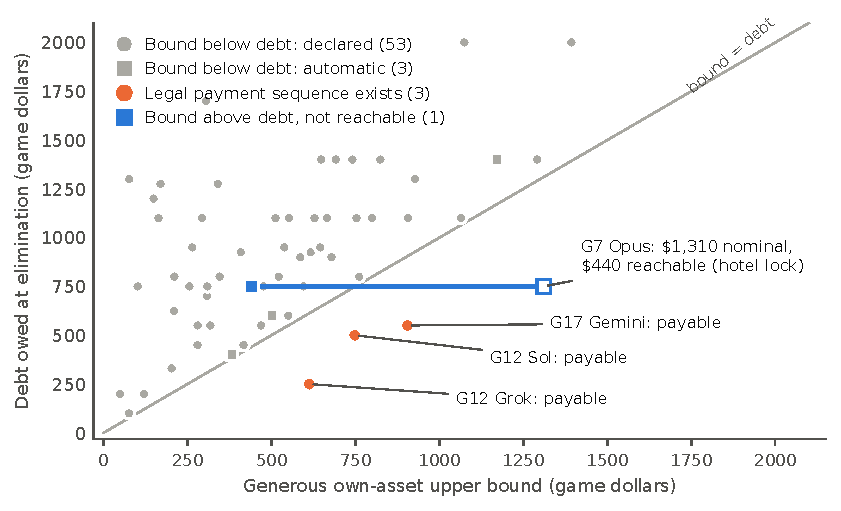
\includegraphics[width=0.86\linewidth]{fig_financing.pdf}
\caption{Debt at elimination against the generous own-asset bound for all sixty eliminations. Points above the diagonal cannot be paid by any sequence of the debtor's own sales and mortgages. For game 7 the open square is the nominal bound and the filled square is the amount actually reachable. The classification concerns payment of the current debt without help. It does not assess earlier decisions or what would have followed.}
\label{fig:financing}
\end{figure}

Four cases have a bound above the debt. Three were payable. In game 12 Sol declares with \$500 owed, and an executed sequence of house sales and mortgages pays it and leaves \$38. Sol's note omits the mortgages that selling its red houses would unlock. In game 17 Gemini declares with \$550 owed, and a similar sequence pays and leaves \$180. The third is Incident~\ref{inc:bankruptcy}. The fourth case runs the other way. In game 7 Opus owes \$750 and holds \$1,310 in nominal value, but its pink group stands at a hotel and two sets of four houses, the bank has no houses left to downgrade the hotel, and the even-selling rule blocks the alternatives. Only \$440 is reachable. Nominal equity is not accessible cash.

At the moment of elimination, then, these systems almost never give up with a way to pay. That is a statement about the last decision only. An unpayable debt says nothing in favor of the purchases, trades and building that led to it, and a payable one does not show the player would have survived much longer.

\IncidentTitle{bankruptcy}{Bankruptcy applied while the response argues for selling}

In game 12, Grok owes Opus \$250 in rent and has \$43. Its pink group holds two, two and three houses. The liquidation menu offers a sale or bankruptcy. The assistant text of Grok's response requests a sale:

\TranscriptQuote{g12-sale}

The private note on the same response ends:

\TranscriptQuote{g12_d249_private_final}

The one tool call in the response is a bankruptcy declaration, with this public message:

\TranscriptQuote{g12_d249_public_bankruptcy}

\IncidentOutcome{The engine applies the bankruptcy and Grok's estate goes to Opus, who wins the game. An executed sequence of five house sales would have paid the \$250 and left \$43.}

\IncidentReading{This is the only one of the 139 text and tool-call disagreements in which the call declared bankruptcy. The elimination was avoidable at the current debt, and the response's own text and note argue for avoiding it. It cannot be read as a decision to surrender. The note's intermediate figures contain errors, so the payment sequence was established independently.}

\IncidentSource{G12 d249, turn 101, standard first attempt with a single tool call. The payment sequence is in the retained certificate suite.}

\subsection{Estates move more property than trades}

A bankrupt player's deeds go to its creditor with their buildings. Figure~\ref{fig:routes} shows the scale of this transfer. Players came to own a complete color group 209 times. Sixty-three of those completions were by trade, 16 by direct purchase, 9 by auction and 121 by estate. Sixty-nine of the estate completions arrive with the final elimination, when play is over. The other 52 arrive while the game is still running, which is nearly as many as trade produces.

\begin{figure}[t]
\centering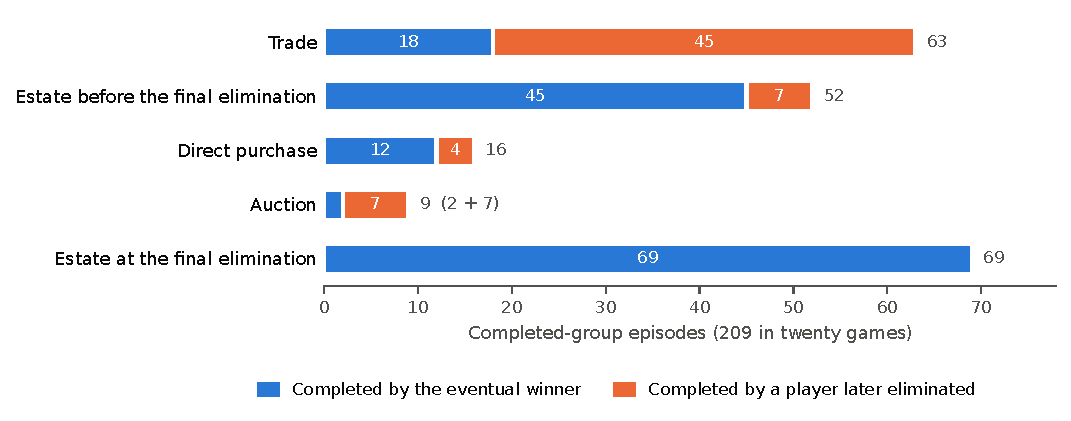
\includegraphics[width=0.86\linewidth]{fig_routes.pdf}
\caption{How complete color groups were assembled, by whether the player who completed the group won that game. Winner status is an endpoint that the same events help produce, so the split describes concentration and is not an estimate of what inheritance contributes to winning.}
\label{fig:routes}
\end{figure}

The two routes go to different players. Of the 63 groups completed by trade, 18 belong to the eventual winner, a little above one in four. Of the 52 groups completed by estate before the final elimination, 45 belong to the eventual winner. In 16 of the 20 games a single player is the creditor in all three eliminations and takes every estate. The winner receives the first estate in 18 games. Of the 227 deeds that change hands through estates before the final elimination, the eventual winner receives 202.

Trade-completed groups still earn most of the rent. Rent paid on complete groups, from completion until loss or game end, totals \$95,278 of the \$121,154 paid in all. Groups completed by trade collect \$57,378 of it and groups completed by direct purchase \$23,070. Groups completed by estate collect \$11,472, and only 14 of the 52 collect any, because estates arrive late. Monopolies assembled by trade and purchase generate the rent that bankrupts rivals, and the estates then concentrate the board in the creditor's hands.

Nothing here measures the effect of inheritance on winning, since the creditor is usually the player who already owned the developed group that caused the bankruptcy. The observation is about the rule. A player who cannot pay transfers a portfolio to one specific rival, and every other player has a stake in which rival that is.

\subsection{Bargaining over who inherits}

The systems act on that stake. The Boardwalk purchase in Section~\ref{sec:cashpoor} was justified by it. In the two incidents below a seller uses the threat of its own bankruptcy as a selling point, and a buyer withdraws terms once the seller is close to it.

\IncidentTitle{insurance}{A deed sold as insurance against a rival's inheritance}

In game 13, Grok has \$35 and stands nine squares before Short Line, where Sol's four railroads would charge \$200. Grok owns the yellow group. One yellow deed, Ventnor Avenue, is unmortgaged and could be mortgaged for \$130. Grok offers its mortgaged Pennsylvania Avenue to Opus for \$200:

\TranscriptQuote{g13-opening-insurance}

Opus, which holds \$1,926, counters at \$130. Its returned explanation values keeping Grok solvent and calls \$200 too high. That reasoning follows Grok's appeal and may simply adopt it. Grok answers:

\TranscriptQuote{g13-seller-counter}

Grok's private note on the same response shows that it knows about the mortgage and prefers not to use it:

\TranscriptQuote{g13-seller-floor}

The reasoning text returned with that response is blunter:

\TranscriptQuote{g13-omission-explanation}

Opus accepts:

\TranscriptQuote{g13-acceptance}

\IncidentOutcome{Opus pays \$200 plus \$16 in mortgage-transfer interest. In the retained exact-prefix check, accepting \$130 and then mortgaging Ventnor gives Grok \$295, enough to pay the rent. Forty-three turns later Grok lands on Short Line with \$49 and nothing left to mortgage, and the yellow group passes to Sol after all. Sol is later eliminated by a \$100 tax it cannot pay, and Opus wins.}

\IncidentReading{The seller prices a deed by the buyer's interest in the seller's survival, and the buyer pays the price. The statement that \$130 leaves Grok \$35 short is true of cash and leaves out a way to pay that Grok's own note records. The \$70 difference between counter and settlement is observed. That the omission caused it is not. The stakes had been framed before the omission, Opus's text never says the cheaper route is impossible, and Grok's note sets its own floor at \$165, which reads as a bargaining position as much as a claim of necessity. The opening probability is also wrong, since Short Line is a 4-in-36 roll from that square. Public misstatement was permitted. The incident establishes that solvency itself was traded and that the protection bought lasted 43 turns.}

\IncidentSource{G13 d250--253, turn 107, and d311, turn 150. Grok's responses are standard first attempts. Opus's are action-only retries without a private note. The excerpt of returned reasoning comes from a 21,134-character text that also contains inconsistent arithmetic. The d252--253 prompts contain one garbled trade-history line, with correct holdings fields.}

\IncidentTitle{withdrawal}{A standing offer withdrawn when the seller is nearly broke}

In game 18, Opus wants Sol's mortgaged Pacific Avenue to complete the green group. It offers \$250, calls the price final, and says on three later decisions that the offer stands. After collecting \$750 in rent from Sol it says so again:

\TranscriptQuote{g18-assurance}

Sol had refused that price as too low. A second \$750 rent then forces Sol to sell its orange buildings and mortgage its remaining red deeds, leaving it \$49. Two larger packages fail, and Sol takes up the advertised price. Opus holds \$2,125:

\TranscriptQuote{g18-invocation}

\TranscriptQuote{g18-withdrawal}

The reasoning returned with Opus's response gives the ground:

\TranscriptQuote{g18-withdrawal-explanation}

\IncidentOutcome{No sale occurs at \$250. Opus later offers \$150 and then \$225, Sol asks for more, and nothing settles. Opus wins the game and is the creditor at Sol's elimination.}

\IncidentReading{The buyer's stated reason for withdrawing is the seller's insolvency. Cash paid to a player about to go bankrupt only delays an estate the payer may receive anyway. Incident~\ref{inc:insurance} shows a third party paying to keep a debtor alive. Here the likely creditor declines to. The record does not show that the offer was insincere when made, or that Sol gave anything up in reliance on it. The game has no object for a standing offer and none of the messages set an expiry.}

\IncidentSource{G18 d421--442. The d431 assurance is in both players' prompts at d441 and d442. Opus's messages are action-only retries, and the explanation is provider-returned text.}

Another blocking purchase ends like the insurance sale. In game 18 Grok buys a mortgaged Illinois Avenue for \$100 from a seller holding \$2, saying this keeps Sol off the red group. Eighteen turns later Grok is bankrupt to Sol, and Illinois completes Sol's reds. A blocking deed protects only while its holder stays solvent, and the debt, not the holder, decides who receives it.

\subsection{The first monopoly and the outcome}

The three parts of the account meet in one tabulation (Table~\ref{tab:cohort}). In each game take the first complete color group. It is completed by trade in 14 games and by direct purchase in 6. Its owner wins 15 of the 20 games. In 12 of those 15 the owner builds on the group in its first management window. In the 5 games the first completer loses, 4 have a first window with no building: one engine default (game 4), two text and tool-call disagreements (games 8 and 20) and one purchase that left too little cash for a house (game 15).

These are twenty dependent games with a selected endpoint, and four of the 15 wins are the block in which seat 2 always bought dark blue. We do not read the table as an effect of building on winning. It shows that the path from first monopoly to development to estates describes most of the games.

\section{Plans, forecasts and repeated errors}
\label{sec:temporal}

The record also contains what the systems said they would do, what they expected of others, and how they responded to rejected actions. This evidence is thinner.

\paragraph{Stated plans meet opportunities unevenly.} An earlier pass read the public message and private note of 240 sampled decisions, three per player per game. A language-model reader marked forward-looking statements about the player's own actions in 59. Most are contingent or open-ended. Eight state a checkable policy of buying a named property on landing there. Following each player to the end of its game, six never get the chance. One is carried out. The eighth meets its opportunity and is not. In game 16 Grok's note includes the plan \InlineQuote{fx-g16-plan}. Fifty-six decisions later it lands on Virginia Avenue with \$371 against a \$160 price. Its note says \InlineQuote{fx-g16-note} Its public message says \InlineQuote{fx-g16-public} The tool call starts an auction, which Gemini wins at \$380. This is one of the eleven Grok decisions whose text buys and whose call auctions. A plan can fail for lack of an opportunity or at the response layer, and neither is a change of mind. Opus's notes are absent in 53 of its 60 sampled decisions, so these counts cannot compare planning across systems.

\paragraph{Some targets are carried across many turns.} In game 9, Sol's note at turn 29 sets a target of three houses on each dark-blue deed as funds arrive. It adds one house the next turn, another at turn 39, and reaches three on each at turn 60 after mortgaging a spare deed. The target is realized through intervening rolls, rents and financing. The chronology does not show that the note caused the result.

\paragraph{Statements about opponents are mostly accounting.} The same reader marked statements about what an opponent could or would do in 36 sampled decisions. Nearly all concern public quantities such as cash, reachable rents and mortgage capacity. Some are checkable and correct. In the Boardwalk purchase of Section~\ref{sec:cashpoor}, Grok's note predicts that Opus cannot survive a light-blue hotel, and four turns later Opus is eliminated owing Gemini \$550. In Incident~\ref{inc:swap}, Sol's third offer answers the objection Grok had stated in public. These show attention to a rival's finances and stated reasons. They are not predictions of hidden beliefs.

\paragraph{An encoding error recurs when feedback is absent, and sometimes when it is present.} The uneven-build rejection of Section~\ref{sec:defaults} occurs in 114 decisions. For each we find the same player's next decision in that game that submits a build plan (Table~\ref{tab:recurrence}). The error recurs at that next submission in 63 of 109 cases. Fifty-four of the 63 are Opus. Its retry had been spent on the refusal, so in 60 of its 61 error decisions no request showed it the validator's message. In the 54 decisions where a corrective request did show the message, the error recurs at 9 of 50 next submissions, and at 2 of 29 when only the first such request in each player-game is counted. These are sequences under changing states with no control condition. The error is usually not repeated once the message has been seen, which is not a measurement of learning.

\begin{table}[t]
\centering\small
\begin{tabular}{lrrr}
\toprule
Uneven-build rejections & Decisions & Later submission & Error repeated\\
\midrule
All & 114 & 109 & 63\\
Validator message shown in a corrective request & 54 & 50 & 9\\
First such request per player and game & 31 & 29 & 2\\
\bottomrule
\end{tabular}
\caption{Recurrence of the uneven-build encoding error at the same player's next build submission in the same game. The populations are nested. Decisions with no later submission are censored. Inherited from the earlier audit.}
\label{tab:recurrence}
\end{table}

\section{Discussion}
\label{sec:discussion}

\subsection{What the account says about an economic agent}

\paragraph{The systems judge a deal partly by what it gives the other side.} This shows in three independent places: the cash terms, which charge for completion in both directions; the responses, which turn against offers that complete the writer's group; and the stated reasons, which name the rival's set, cash or survival. Studies of bilateral bargaining report that language models anchor on opening offers and concede without compensation~\cite{cosentino2026counterparty,shah2025rationalis}. The setting here has four players, a single winner and full visibility of everyone's cash and holdings, and in it no system treats agreement as the default. We cannot say the systems refuse the right offers. Incident~\ref{inc:swap} shows a refusal that was coherent, checkable and followed by the refuser's bankruptcy.

\paragraph{The bargain's value is realized or lost in execution.} Two systems turned negotiated monopolies into houses almost every time. Two did not, and for 17 of 20 unbuilt groups the reason lies in the acquisition terms or the response path. The largest single loss came from a provider refusal that removed the one retry in which a build plan could have been corrected. Scoring these games by wins would attribute that to the model, and scoring them by deals closed would miss it. Results from one harness should not be read as properties of the model inside it, a point made elsewhere with matched harness comparisons and with reliability analyses of agent leaderboards~\cite{zhang2026dece,hardy2026reliability}.

\paragraph{When default transfers assets, solvency becomes a traded good.} Under intact creditor inheritance a bankrupt player hands a portfolio to one rival, and estates completed 52 groups during play. The systems bargained over this. A seller offered its own survival as insurance, buyers paid above their limits to keep deeds out of estates, and a likely creditor withdrew an offer that would have prolonged a debtor's life. Cash-poor holders released the deeds that liquid holders refused to sell, without becoming more agreeable. Several protective purchases were undone by a later bankruptcy. The Vending-Bench Arena study reports that misaligned messages become more likely when an agent's inventory is low~\cite{li2026arena}. Our cash-poor counts have no comparable outcome measure, but both records suggest that scarcity deserves separate attention when agents trade.

\subsection{Coverage of the broader questions}

The study was motivated by eight questions about strategic agents and three questions that cut across them. Table~\ref{tab:coverage} states, for each, what this cohort supports and at what level. ``Census'' means a count over a complete population of recorded events. ``Cases'' means checked incidents with no rate.

\begin{table}[p]
\centering\footnotesize
\renewcommand{\arraystretch}{1.12}
\begin{tabularx}{\linewidth}{@{}L{2.55cm}YL{1.75cm}L{3.5cm}@{}}
\toprule
Question & What this cohort supports & Level & Not established\\
\midrule
1. Strategic reasoning and rationality & Completion is priced by both sides. Offers that complete the writer's group are mostly refused. Recipients decline their own monopoly citing the rival's gain (Incident~\ref{inc:swap}). Payable debts are abandoned in 3 of 60 eliminations. & Census and cases & That any choice maximized the chance of winning. Regret or exploitability.\\
2. Opponent modeling & Notes and messages reason about rivals' cash, collateral and building capacity. Some forecasts are checkable and correct. A proposer answers a stated objection. & Cases & Accuracy over a defined set of forecasts. Inference about hidden beliefs.\\
3. Cooperation, negotiation and deception & All 920 responses with ownership consequences. Four declining styles at similar acceptance. A bluffed limit, an omitted financing route, a withdrawn offer, a coordination appeal. & Census for actions, cases for speech & Negotiation effectiveness, fairness, a deception rate, persuasion, absence of agreement bias.\\
4. Long-horizon planning and memory & The path from completion to building to rent for every traded monopoly. Post-trade cash against house cost. One target carried over 31 turns, one plan lost at the response layer. Memory conditions documented. & Census of trajectories, cases for plans & A rate of plan completion. Any benefit of memory.\\
5. Adaptability and learning & The encoding error recurs in 9 of 50 next submissions after the validator message was shown. & Observed sequences & Learning caused by feedback. Adaptation to an opponent.\\
6. Economic decisions and risk & Financing feasibility at all 60 eliminations. Nominal equity is not accessible cash (game 7). Who pays for completion, and how much. Spending and receipts by unit. & Census & The ex ante value of a purchase. Optimal reserves. Risk-adjusted return.\\
7. Emergent and collective behavior & Estates concentrate property. One creditor takes all three estates in 16 games. Cash-poor holders release blocking deeds. One open boycott appeal. & Census of flows, one case & How often coalitions form or last. Any effect of coordination.\\
8. Validity and generalization & Conditions that change what records mean are stated and counted. Ledgers reconcile with the engine. Seat and seed dependence is visible in three blocks. & Internal consistency & Transfer to other opponents, rules or runs. Any ranking.\\
\midrule
A. Strategic talk and strategic action & Text and applied action disagree in 139 Grok decisions, including a bankruptcy. Stated plans are carried out, lost at the response layer, or never tested. & Census for one system, cases & A general relation between explanation quality and action quality.\\
B. General and multi-agent capability & Not evaluated. Four configurations and no independent capability measure. & None & The relationship itself.\\
C. Skill, luck and exploitation & Seven games follow the seat that bought an early monopoly from the bank, whichever system sat there. Four follow one system across seats. Specific execution failures are located. & Descriptive & A decomposition of winning into skill, chance and opponents' errors.\\
\bottomrule
\end{tabularx}
\caption{What the cohort supports for each motivating question. Levels describe the evidence, not the systems.}
\label{tab:coverage}
\end{table}

Three rows need a sentence more. On question A, the record separates four things that a transcript blurs: a statement about the board, a stated plan, a submitted action and the action the engine applied. They can each be right or wrong independently. The Opus build plans were sound as plans and invalid as submissions, and Grok's game-12 response argued correctly for selling houses while its tool call declared bankruptcy. Neither case says anything simple about whether the model is strategic.

On question B, the honest answer is that this study has nothing to add. Others report that larger models do not consistently win more Monopoly games~\cite{wu2026agentmonopoly} and that performance rank does not predict misaligned communication~\cite{li2026arena}. Four heterogeneous configurations cannot test either claim.

On question C, the seed blocks give an unusually direct view. The same dice put the same early monopoly in the same seat four times, and four different systems won from it. In another block one system won from all four seats. Both luck and system differences are visible in a twenty-game cohort, and their shares cannot be estimated from it.

\section{Related work}
\label{sec:related}

\paragraph{Bargaining by language models.} NegotiationArena studies bilateral scenarios and shows that bargaining tactics change outcomes~\cite{bianchi2024negotiationarena}. Abdelnabi et al.\ build scorable multi-party, multi-issue negotiations that include greedy and adversarial players~\cite{abdelnabi2024stakeholders}. More recent bilateral studies find that models represent a counterparty's preferences accurately without converting that into better agreements, and that they anchor at the extremes of the bargaining zone~\cite{cosentino2026counterparty,shah2025rationalis}. In a market with one seller and several buyers, standard models are reported to fixate on the current highest bid instead of exploring the buyer pool~\cite{liu2026multibuyer}. Cattle Trade combines auctions, bluffing and bargaining in one game and finds that coherent spending predicts rank better than any single skill~\cite{muller2026cattletrade}. These studies score outcomes against a defined utility, which this paper does not. We add bargaining inside a long game, where the traded asset is worth what its buyer can later build on it and each offer can be described by what it would complete for each side.

\paragraph{Long-horizon economic agents.} Vending-Bench and CEO-Bench evaluate sustained operation of a simulated business, and in CEO-Bench every model falls below a rule-based baseline~\cite{backlund2025vendingbench,chen2026ceobench}. The Vending-Bench Arena communication study checks 2,583 inter-agent emails against simulator state, replicates its classifier with other judge families, and ties misaligned messages to scarcity and to the counterparty's behavior~\cite{li2026arena}. FinBoardBench evaluates financial decisions in three board games including Monopoly and reports that models favor acquiring assets over keeping liquidity~\cite{hu2026finboardbench}. AgentMonopoly studies the same underlying game across four model families and two sizes, with persona interventions, and reports differences in how often models trade and how they manage cash~\cite{wu2026agentmonopoly}. Both record invalid outputs and fallbacks. In the versions inspected for the earlier draft, FinBoardBench returns buildings to the bank when a creditor inherits, AgentMonopoly transfers them intact as this engine does, and AgentMonopoly's trade interface accepts or rejects a single offer where ours allows counters. Our account differs in grain. It follows every offer, every traded monopoly and every bankruptcy to its consequence and identifies the response path behind each failure to build.

\paragraph{Strategic and social game benchmarks.} GTBench, GAMA-Bench and SPIN-Bench measure strategic reasoning across many games~\cite{duan2024gtbench,huang2025gamabench,yao2025spinbench}. Agent Island ranks 49 models over 999 elimination games and finds same-provider favoritism in votes~\cite{murphy2026agentisland}. MINDGAMES reports fragile rule-following and uneven leaderboard validity from a large competition~\cite{wang2026mindgames}. CoopEval compares mechanisms that sustain cooperation in social dilemmas~\cite{tewolde2026coopeval}. DECE evaluates model and harness configurations across ten Eurogames and shows that the same model performs differently under different harnesses~\cite{zhang2026dece}. These designs buy statistical power with many matches. Ours reconstructs a few long games completely and cannot support the rankings theirs can.

\paragraph{Evaluating configured systems.} The Holistic Agent Leaderboard argues for evaluating complete agent systems and inspecting their logs~\cite{kapoor2026hal}. Hardy et al.\ show that rankings of fixed model and scaffold systems are reliable while rankings of underlying models are much less so~\cite{hardy2026reliability}. AgentBoard reports process metrics beyond final success~\cite{ma2024agentboard}. Yang et al.\ audit leaderboard claims with matched controls and scorer validation~\cite{yang2026measurementfirst}. Our legal-sequence checks serve the behavioral description. We have not evaluated them as an auditing method on held-out cases.

\paragraph{Commitments, deception and explanations.} Work on agent promises separates infeasible commitments from feasible ones that are not kept and asks who may release a promise~\cite{empty_commitments_v2,commitment_standing,shi2026cheaptalk}. Designed settings elicit collusion against a verification protocol in most trajectories~\cite{shi2026emergentcollusion}, and MASK separates honesty from accuracy~\cite{ren2025mask}. The norm matters for comparison. Our prompt permits public deception, AgentMonopoly's encourages bluffing while prohibiting messages that contradict the action, and the Arena study applies an external taxonomy to agents given no conduct instruction. The same sentence can be a violation in one and a legal move in another. Work on explanation faithfulness and monitorability motivates our caution about text channels~\cite{turpin2023unfaithful,lanham2023faithfulness,korbak2025monitorability}.

\section{Limitations}
\label{sec:limitations}

\paragraph{A small, dependent cohort.} Twenty games come from five seeds. Decisions within a game share a board, rotations within a block share early dice, and the four cyclic rotations cover four of the 24 possible seat orders. Every system faced the same three opponents, whose model names were visible. The counts are censuses of this cohort. They carry no confidence intervals and support no ranking, seat effect or forecast for other opponents.

\paragraph{Unequal conditions.} Opus played 95 percent of its decisions through an action-only recovery path whose trigger is unknown. Grok's text and tool calls disagree in 139 decisions for reasons the record cannot locate. Token use differs by a factor of thirty across systems. Thirty percent of prompts contain a garbled line of trade history. None of these was assigned as a treatment, so comparisons across systems are comparisons across these conditions.

\paragraph{One rule set.} Intact creditor inheritance, per-entry even-building checks and a bankruptcy option that is always on the menu shape the results. The inheritance findings in particular describe this variant. The engine also overcharges some mortgage redemptions by one dollar through a floating-point ceiling, which the replay faithfully reproduces. Replay shows that the record is consistent with the implementation. It does not certify the implementation against an independent statement of the rules.

\paragraph{Observation without intervention.} Offers differ in price, contents, responder and thread position within every category we tabulate, so no contrast estimates an effect. The cash-poor threshold is arbitrary, and splits by eventual winner condition on an outcome the same events produce. No trade, refusal, purchase or bankruptcy is shown to be good or bad play, because no reference policy or continuation value was computed.

\paragraph{Text.} Private notes are absent for most Opus decisions, returned reasoning is available unevenly, and no channel is privileged. Semantic codes were assigned by language models that overlap with the participants in model or developer, with one partly unblinded second reading and no human labels. The incidents were selected to illustrate mechanisms, and most involve Grok because its channels are the most observable.

\paragraph{Checks inherited by this draft.} The engine executions behind the payable and unpayable classifications, the rebuilt construction plans and the replay were performed in an earlier audit, and this draft re-tabulated their retained outputs without rerunning them. The negative classification rests on an arithmetic bound in 56 cases and on an exhaustive search of a one-action graph in one. A general search over bundled building sales is not supported by the retained checker. Appendix~\ref{app:provenance} separates what was recounted here from what was inherited.

\paragraph{No new evaluation.} The study is confined to existing records. Whether the bargaining is effective, whether feedback produces learning, and whether any of this transfers to other opponents or rules are questions that need interventions or new runs.

\section{Conclusion}

In twenty complete games, four configured LLM systems bargained hard, built unevenly and were sorted by bankruptcy. They priced the completion of a color group on both sides of a trade, refused or repriced most offers that would arm the proposer, and released blocking deeds mainly when short of cash. Two systems converted nearly every negotiated monopoly into houses. Two lost most of that value to illiquid purchases, to a refusal that consumed the only retry, and to tool calls that contradicted their own text. Nearly every bankruptcy was unpayable when it came, and under intact inheritance the estates completed almost as many monopolies during play as trade did and delivered them to a single creditor in most games.

For evaluation, the practical consequence is that a multiplayer economic game has at least three places to look, and they can disagree. The record of deals, the record of what was built and the record of who inherited each tell a different part of how these games ended. A win count, a deal count or a striking transcript read alone would have misdescribed all four systems.

\begingroup
\small
\bibliographystyle{plainnat}
\bibliography{references}
\endgroup
\clearpage
\appendix
% Generated by tools/make_tables.py; do not edit.
\newcommand{\CohortRows}{%
1 & 1 & 1 & 216 & Gemini & 3 & Gemini & light blue & trade & 40 & yes & yes\\
2 & 1 & 2 & 102 & Gemini & 2 & Gemini & dark blue & trade & 18 & yes & yes\\
3 & 1 & 3 & 283 & Gemini & 1 & Gemini & dark blue & trade & 17 & yes & yes\\
4 & 1 & 4 & 166 & Grok & 1 & Sol & pink & trade & 62 & no & no\\
5 & 2 & 1 & 170 & Sol & 2 & Sol & green & trade & 94 & yes & yes\\
6 & 2 & 2 & 126 & Sol & 1 & Sol & orange & trade & 74 & yes & yes\\
7 & 2 & 3 & 150 & Sol & 4 & Sol & dark blue & trade & 67 & yes & yes\\
8 & 2 & 4 & 139 & Sol & 3 & Grok & orange & trade & 74 & no & no\\
9 & 3 & 1 & 88 & Sol & 2 & Sol & dark blue & purchase & 29 & yes & yes\\
10 & 3 & 2 & 75 & Gemini & 2 & Gemini & dark blue & purchase & 29 & yes & yes\\
11 & 3 & 3 & 145 & Grok & 2 & Grok & dark blue & purchase & 29 & no & yes\\
12 & 3 & 4 & 166 & Opus & 2 & Opus & dark blue & purchase & 29 & yes & yes\\
13 & 4 & 1 & 185 & Opus & 1 & Opus & orange & purchase & 47 & no & yes\\
14 & 4 & 2 & 110 & Sol & 1 & Sol & orange & purchase & 47 & yes & yes\\
15 & 4 & 3 & 114 & Gemini & 1 & Opus & dark blue & trade & 24 & no & no\\
16 & 4 & 4 & 386 & Sol & 3 & Sol & brown & trade & 49 & yes & yes\\
17 & 5 & 1 & 118 & Sol & 2 & Opus & red & trade & 51 & yes & no\\
18 & 5 & 2 & 197 & Opus & 4 & Opus & brown & trade & 39 & no & yes\\
19 & 5 & 3 & 175 & Gemini & 1 & Gemini & light blue & trade & 31 & yes & yes\\
20 & 5 & 4 & 115 & Gemini & 4 & Grok & red & trade & 22 & no & no\\}
\newcommand{\CellByRecipientRows}{%
Sol & Writer only & 83 & 2 & 50 & 31\\
 & Recipient only & 30 & 6 & 21 & 3\\
 & Both & 8 & 1 & 6 & 1\\
 & Neither & 114 & 21 & 63 & 30\\
\addlinespace
Gemini & Writer only & 76 & 4 & 9 & 63\\
 & Recipient only & 31 & 6 & 10 & 15\\
 & Both & 34 & 6 & 12 & 16\\
 & Neither & 100 & 10 & 5 & 85\\
\addlinespace
Opus & Writer only & 52 & 7 & 42 & 3\\
 & Recipient only & 42 & 5 & 31 & 6\\
 & Both & 11 & 2 & 7 & 2\\
 & Neither & 83 & 15 & 60 & 8\\
\addlinespace
Grok & Writer only & 78 & 6 & 10 & 62\\
 & Recipient only & 37 & 7 & 16 & 14\\
 & Both & 28 & 1 & 10 & 17\\
 & Neither & 111 & 14 & 41 & 56\\}
\newcommand{\CellByBlockRows}{%
1 & 63 & 1 & 27 & 35 & 39 & 9 & 13 & 17\\
2 & 32 & 2 & 9 & 21 & 7 & 2 & 4 & 1\\
3 & 57 & 5 & 24 & 28 & 24 & 1 & 19 & 4\\
4 & 64 & 7 & 22 & 35 & 34 & 7 & 19 & 8\\
5 & 73 & 4 & 29 & 40 & 36 & 5 & 23 & 8\\}
\newcommand{\CellByGameRows}{%
1 & 25 & 0 & 8 & 17 & 9 & 2 & 3 & 4\\
2 & 10 & 0 & 6 & 4 & 9 & 3 & 4 & 2\\
3 & 6 & 1 & 4 & 1 & 10 & 2 & 2 & 6\\
4 & 22 & 0 & 9 & 13 & 11 & 2 & 4 & 5\\
5 & 10 & 0 & 0 & 10 & 0 & 0 & 0 & 0\\
6 & 3 & 0 & 0 & 3 & 1 & 0 & 0 & 1\\
7 & 9 & 0 & 8 & 1 & 4 & 2 & 2 & 0\\
8 & 10 & 2 & 1 & 7 & 2 & 0 & 2 & 0\\
9 & 12 & 0 & 6 & 6 & 7 & 1 & 5 & 1\\
10 & 11 & 1 & 6 & 4 & 3 & 0 & 3 & 0\\
11 & 11 & 1 & 2 & 8 & 5 & 0 & 4 & 1\\
12 & 23 & 3 & 10 & 10 & 9 & 0 & 7 & 2\\
13 & 17 & 2 & 6 & 9 & 11 & 2 & 6 & 3\\
14 & 16 & 2 & 7 & 7 & 7 & 1 & 5 & 1\\
15 & 13 & 0 & 6 & 7 & 9 & 2 & 4 & 3\\
16 & 18 & 3 & 3 & 12 & 7 & 2 & 4 & 1\\
17 & 27 & 2 & 9 & 16 & 14 & 1 & 10 & 3\\
18 & 18 & 1 & 9 & 8 & 12 & 1 & 6 & 5\\
19 & 10 & 0 & 4 & 6 & 4 & 2 & 2 & 0\\
20 & 18 & 1 & 7 & 10 & 6 & 1 & 5 & 0\\}
\newcommand{\CellByPositionRows}{%
Writer only & 187 & 3 & 46 & 138 & 102 & 16 & 65 & 21\\
Recipient only & 51 & 2 & 18 & 31 & 89 & 22 & 60 & 7\\
Both & 48 & 3 & 11 & 34 & 33 & 7 & 24 & 2\\
Neither & 238 & 24 & 62 & 152 & 170 & 36 & 107 & 27\\}
\newcommand{\CellCashRows}{%
Writer only & 289 & 238 & 40 & 11 & 200 & 286 & 16 & 111 & 159\\
Recipient only & 140 & 5 & 0 & 135 & -350 & 139 & 24 & 78 & 37\\
Both & 81 & 15 & 19 & 47 & -100 & 81 & 10 & 35 & 36\\
Neither & 408 & 234 & 28 & 146 & 100 & 401 & 56 & 168 & 177\\}
\newcommand{\CashPoorRows}{%
\$50 & 47 & 8 & 30 & 9 & 70 & 12 & 28 & 30 & 20 & 14\\
\$100 & 85 & 12 & 55 & 18 & 132 & 18 & 52 & 62 & 30 & 21\\
\$150 & 101 & 15 & 64 & 22 & 158 & 21 & 62 & 75 & 36 & 22\\
\$200 & 117 & 19 & 69 & 29 & 171 & 21 & 70 & 80 & 40 & 24\\}
\newcommand{\NeverLegalRows}{%
G1 d289 & Grok & orange & \$100 & \$18 & \$229 & \$100 & deed arrived mortgaged\\
G1 d309 & Grok & dark blue & \$100 & \$20 & \$219 & \$200 & deed arrived mortgaged\\
G8 d262 & Opus & brown & \$120 & \$3 & \$507 & \$50 & deed arrived mortgaged\\
G12 d229 & Opus & light blue & \$25 & \$6 & \$19 & \$50 & deed arrived mortgaged\\
G14 d203 & Grok & dark blue & \$200 & \$18 & \$584 & \$200 & deed arrived mortgaged\\
G15 d56 & Opus & dark blue & \$750 & \$0 & \$158 & \$200 & cash below one house\\
G16 d229 & Grok & orange & \$170 & \$10 & \$483 & \$100 & deed arrived mortgaged\\
G16 d247 & Opus & dark blue & \$150 & \$18 & \$268 & \$200 & deed arrived mortgaged\\
G20 d296 & Opus & dark blue & received \$100 & \$0 & \$125 & \$200 & cash below one house\\}
\newcommand{\EliminationRows}{%
1 & Gemini & Opus$\to$Gemini & \$550 & \$318 & Sol$\to$Gemini & \$200 & \$121 & Grok$\to$Gemini & \$1,275 & \$170\\
2 & Gemini & Opus$\to$Gemini & \$1,300 & \$927 & Sol$\to$Gemini & \$1,300 & \$77 & Grok$\to$Gemini & \$330 & \$203\\
3 & Gemini & Opus$\to$Gemini & \$1,100 & \$552 & Sol$\to$Gemini & \$2,000 & \$1,074 & Grok$\to$Gemini & \$925 & \$617\\
4 & Grok & Sol$\to$Grok & \$550 & \$469 & Gemini$\to$Grok & \$750 & \$256 & Opus$\to$Grok & \$625 & \$210\\
5 & Sol & Grok$\to$Sol & \$900 & \$586 & Gemini$\to$Sol & \$1,200 & \$149 & Opus$\to$Sol & \$1,100 & \$799\\
6 & Sol & Grok$\to$Sol & \$750 & \$595 & Opus$\to$Sol & \$750 & \$102 & Gemini$\to$Sol & \$800 & \$211\\
7 & Sol & Grok$\to$Sol & \$1,400 & \$1,291 & Gemini$\to$Sol & \$1,400 & \$741 & Opus$\to$Sol$^{h}$ & \$750 & \$1,310\\
8 & Sol & Gemini$\to$Sol & \$700 & \$308 & Grok$\to$Sol & \$1,100 & \$666 & Opus$\to$Sol & \$750 & \$309\\
9 & Sol & Gemini$\to$Sol & \$1,100 & \$913 & Grok$\to$Sol & \$1,400 & \$1,171 & Opus$\to$Sol & \$1,400 & \$824\\
10 & Gemini & Sol$\to$Gemini & \$1,400 & \$692 & Opus$\to$Gemini & \$1,400 & \$648 & Grok$\to$Gemini & \$600 & \$509\\
11 & Grok & Gemini$\to$Grok & \$1,100 & \$1,064 & Opus$\to$Grok & \$1,700 & \$306 & Sol$\to$Grok & \$1,100 & \$753\\
12 & Opus & Sol$\to$Opus$^{p}$ & \$500 & \$748 & Grok$\to$Opus$^{p}$ & \$250 & \$613 & Gemini$\to$Opus & \$1,100 & \$164\\
13 & Opus & Gemini$\to$Opus & \$950 & \$538 & Grok$\to$Sol & \$200 & \$49 & Sol$\to$bank & \$100 & \$76\\
14 & Sol & Opus$\to$Sol & \$800 & \$346 & Gemini$\to$Sol & \$800 & \$522 & Grok$\to$Sol & \$1,100 & \$907\\
15 & Gemini & Grok$\to$Gemini & \$800 & \$761 & Opus$\to$Gemini & \$950 & \$645 & Sol$\to$Gemini & \$450 & \$280\\
16 & Sol & Opus$\to$Gemini & \$550 & \$280 & Grok$\to$Sol & \$1,100 & \$628 & Gemini$\to$Sol & \$2,000 & \$1,393\\
17 & Sol & Gemini$\to$Sol$^{p}$ & \$550 & \$905 & Opus$\to$Sol & \$1,100 & \$293 & Grok$\to$Sol & \$750 & \$476\\
18 & Opus & Gemini$\to$Opus & \$400 & \$382 & Grok$\to$Sol & \$950 & \$264 & Sol$\to$Opus & \$900 & \$679\\
19 & Gemini & Grok$\to$Gemini & \$600 & \$502 & Opus$\to$Gemini & \$925 & \$409 & Sol$\to$Gemini & \$1,100 & \$512\\
20 & Gemini & Grok$\to$Opus & \$450 & \$417 & Opus$\to$Sol & \$600 & \$550 & Sol$\to$Gemini & \$1,275 & \$340\\}

\section{Cohort and units}
\label{app:cohort}

Table~\ref{tab:cohort} lists the twenty games. Decision identifiers are zero-based within a game, so G20 d1 is that game's second decision. A turn can contain several decisions by the same player. Games 1 to 4 and games 5 to 20 were run from two source revisions. The earlier inspection of the difference found changes to campaign concurrency, application, documentation and test files and none to engine, prompt, resolver, player-configuration or gateway-client files.

\begin{table}[H]
\centering\footnotesize
\begin{tabular}{rrrrlr@{\hskip 14pt}llrrll}
\toprule
 & & & & & & \multicolumn{6}{c}{First complete color group in the game}\\
\cmidrule(l){7-12}
Game & Block & Rot. & Turns & Winner & Seat & Owner & Group & Route & Turn & Built & Owner won\\
\midrule
\CohortRows
\bottomrule
\end{tabular}
\caption{The cohort. Block is the shared seed (seeds 751774554, 2506298840, 2573692901, 3648314310 and 2766649504 for blocks 1 to 5). ``Built'' is whether the owner built on the group in its first management window. Seats and rotations are one-based. Re-tabulated for this draft from the cohort export and the completion ledger.}
\label{tab:cohort}
\end{table}

\begin{table}[H]
\centering\small
\begin{tabularx}{\linewidth}{L{3.3cm}Y}
\toprule
Unit & Meaning\\
\midrule
Attempt & One saved provider response, including a refusal or an invalid output.\\
Decision & One engine menu resolved into one applied action. It can contain several attempts.\\
Offer & One trade proposal or counter awaiting a response. The writer is the author of the current terms.\\
Settlement & Accepted terms applied atomically, with both directions and mortgage-transfer interest.\\
Completion episode & One period in which a player owns every deed of a color group, from the completing acquisition to loss or game end.\\
First management window & The owner's first turn with an optional-management menu after a completion, including every management decision in that turn.\\
Spending unit & One player's own house and hotel expenditure on one color group in one game.\\
Elimination & One bankruptcy, declared or automatic.\\
\bottomrule
\end{tabularx}
\caption{Units of analysis. They are not interchangeable denominators.}
\label{tab:units}
\end{table}

\section{What was checked for this draft}
\label{app:provenance}

Tables~\ref{tab:provenance} and~\ref{tab:inherited} give the status of each group of quantities. \textbf{R} means recounted for this draft from the canonical decision logs. \textbf{T} means re-tabulated for this draft from a retained ledger, whose construction and agreement with the engine were established by the earlier audit. \textbf{I} means inherited from the earlier audit without recomputation. The scripts are in \artifact{tools/} and their outputs in \artifact{data/} of this draft's folder. No script calls a model or runs the game engine.

\begin{table}[H]
\centering\footnotesize
\renewcommand{\arraystretch}{1.1}
\begin{tabularx}{\linewidth}{@{}YcL{5.6cm}@{}}
\toprule
Quantity & Status & Source for this draft\\
\midrule
Decisions and attempts per system; refusals by game; 66 defaults by system and game; action counts & R & \artifact{tools/census_decisions.py} over all twenty \artifact{decisions.jsonl}\\
Offer responses by completion category; cash direction; breakdowns by recipient, block, game and thread position; response styles & T & \artifact{tools/retab_offers.py} on \artifact{agenda_offers.json}\\
Cash-poor offers and settlements, with thresholds & T (new) & \artifact{tools/retab_distress.py}\\
Join of Grok text and tool-call disagreements to threads and responses & T (new) & \artifact{tools/retab_conflicts.py} on \artifact{resolution_conditions.json}\\
Completion episodes by route and winner; rent by route and owner; first-window outcomes; post-trade cash; first completion per game & T & \artifact{tools/retab_economy.py} on the phase-1 episode ledger, \artifact{first_management_windows.json} and \artifact{agenda_offers.json}\\
Rent per episode & T, cross-checked & Episode ledger against \artifact{agenda_flows.json}: 209 of 209 agree\\
Elimination classes, shortfalls, order and estate recipients & T & \artifact{t06_eliminations.json}, \artifact{certificate_results.json}, \artifact{agenda_flows.json}\\
All excerpts & R & \artifact{tools/build_quotes.py}: 28 retained fields and 30 spans re-checked against canonical files; 14 new quotes extracted from them\\
Instruction text quoted in Section~\ref{sec:setup} & R & Arena source and one saved standard and action-only prompt\\
Spending units by system & T & \artifact{t05_spending_units.json}\\
Build rule for mortgaged groups; rent doubling on a complete group & R & Engine source, read only\\
\bottomrule
\end{tabularx}
\caption{Quantities recounted or re-tabulated for this draft. Retained ledgers are in the shared \texttt{data/} folder two levels above this draft unless noted.}
\label{tab:provenance}
\end{table}

\begin{table}[H]
\centering\footnotesize
\renewcommand{\arraystretch}{1.1}
\begin{tabularx}{\linewidth}{@{}YcL{5.6cm}@{}}
\toprule
Quantity & Status & Source\\
\midrule
Engine executions: payment sequences, rebuilt build plans, the game-7 search, full replay & I & 126-case certificate suite of 29 October\\
Reconciliation of 6,989 states and 113 settlements; 50,918 events & I & Earlier audit\\
Trade-history formatter and timeline-omission counts; memory-window counts & I & Earlier audit\\
Negotiation propensity per eligible turn; repeat-pair threads & I & \artifact{t02_negotiation.json}, \artifact{agenda_negotiation.json}\\
Uneven-build recovery and recurrence tables; 663 end-of-turn provenance & I & \artifact{t07_build_recovery.json}, \artifact{agenda_recurrence.json}, \artifact{resolution_conditions.json}\\
Semantic codes: 74 rejection reasons; 240-decision sample & I & Two and one language-model readings respectively\\
Token, latency and source-revision statements & I & Earlier audit\\
Incident facts outside the quoted spans and ledgers (event numbers, exact-prefix alternatives, recipient-prompt checks) & I & Bounded source reviews of 29 October\\
\bottomrule
\end{tabularx}
\caption{Quantities inherited from the earlier audit without recomputation.}
\label{tab:inherited}
\end{table}

\section{Bargaining tables}
\label{app:bargaining}

All tables in this appendix are generated from the offer ledger by this draft's scripts. ``Writer only'' means the offer would newly complete a color group for its writer and not for its recipient. Counts are acceptance-legal offers unless stated.

\begin{table}[H]
\centering\footnotesize
\setlength{\tabcolsep}{4.5pt}
\begin{tabular}{lrrrrrrrrr}
\toprule
 & \multicolumn{5}{c}{Net cash, writer to recipient} & \multicolumn{4}{c}{Without disagreeing responses}\\
\cmidrule(lr){2-6}\cmidrule(l){7-10}
Would complete & Offers & Writer pays & None & Recip.\ pays & Median & Offers & Accept & Counter & Reject\\
\midrule
\CellCashRows
\bottomrule
\end{tabular}
\caption{Cash direction by completion category, and responses after removing the eleven trade responses in which Grok's text and tool call named different actions. Medians are in game dollars, positive when the writer pays.}
\label{tab:cellcash}
\end{table}

\begin{table}[H]
\centering\small
\begin{tabular}{llrrrr}
\toprule
Recipient & Would complete & Offers & Accept & Counter & Reject\\
\midrule
\CellByRecipientRows
\bottomrule
\end{tabular}
\caption{Responses by recipient and completion category. The rejection contrast between writer-only and recipient-only offers holds for Sol, Gemini and Grok and not for Opus.}
\label{tab:cellrecipient}
\end{table}

\begin{table}[H]
\centering\small
\begin{tabular}{lrrrrrrrr}
\toprule
 & \multicolumn{4}{c}{First offer of a thread} & \multicolumn{4}{c}{Later offer}\\
\cmidrule(lr){2-5}\cmidrule(l){6-9}
Would complete & Offers & Accept & Counter & Reject & Offers & Accept & Counter & Reject\\
\midrule
\CellByPositionRows
\bottomrule
\end{tabular}
\caption{Responses by position in the thread.}
\label{tab:cellposition}
\end{table}

\begin{table}[H]
\centering\small
\begin{tabular}{rrrrrrrrr}
\toprule
 & \multicolumn{4}{c}{Writer only} & \multicolumn{4}{c}{Recipient only}\\
\cmidrule(lr){2-5}\cmidrule(l){6-9}
Block & Offers & Accept & Counter & Reject & Offers & Accept & Counter & Reject\\
\midrule
\CellByBlockRows
\bottomrule
\end{tabular}
\caption{The two one-sided categories by seed block.}
\label{tab:cellblock}
\end{table}

\begin{table}[H]
\centering\small
\begin{tabular}{rrrrrrrrr}
\toprule
 & \multicolumn{4}{c}{Writer only} & \multicolumn{4}{c}{Recipient only}\\
\cmidrule(lr){2-5}\cmidrule(l){6-9}
Game & Offers & Accept & Counter & Reject & Offers & Accept & Counter & Reject\\
\midrule
\CellByGameRows
\bottomrule
\end{tabular}
\caption{The two one-sided categories by game. Game 5 has no recipient-only offer. The rejection share is higher for writer-only offers in 17 of the other 19 games, equal in game 6 and lower in game 3.}
\label{tab:cellgame}
\end{table}

\begin{table}[H]
\centering\small
\begin{tabular}{lrrrrrrrrrr}
\toprule
 & \multicolumn{4}{c}{Cash offered} & \multicolumn{4}{c}{Cash requested} & \multicolumn{2}{c}{Settlements}\\
\cmidrule(lr){2-5}\cmidrule(lr){6-9}\cmidrule(l){10-11}
Below & Offers & Acc. & Ctr. & Rej. & Offers & Acc. & Ctr. & Rej. & All & Completing\\
\midrule
\CashPoorRows
\bottomrule
\end{tabular}
\caption{Sensitivity of the cash-poor tabulations to the threshold. A side is cash-poor when its cash before the offer is below the threshold. ``Cash offered'' counts offers of net cash to a cash-poor recipient, and ``cash requested'' counts requests for net cash written by a cash-poor player. The last two columns count settlements in which the net cash receiver was cash-poor and, among those, the ones in which the paying side completed a color group.}
\label{tab:cashpoorsens}
\end{table}

The 30 settlements with a seller under \$100 involve Opus as seller 16 times, Sol 7, Grok 5 and Gemini 2, across 15 games. Nine of the 30 sellers won their game. The median time from such a sale to the seller's elimination, among the 21 sellers later eliminated, is 25 turns, and 7 were eliminated within ten turns.

For the opening of negotiations, the earlier audit counts own turns on which a proposal was legal: 834 for Sol, 766 for Gemini, 660 for Opus and 676 for Grok, with proposals on 83, 16, 160 and 106 of them. Sixty-four of Grok's 136 threads, spread over all twenty games, begin with a tool call that proposed while the text named another action.

\section{Development, insolvency and estate tables}
\label{app:economy}

\subsection{Completions that could not be built on}

\begin{table}[H]
\centering\footnotesize
\setlength{\tabcolsep}{4pt}
\begin{tabular}{lllrrrrl}
\toprule
Settlement & Buyer & Group & Net cash paid & Interest & Cash after & House & Why building was not legal\\
\midrule
\NeverLegalRows
\bottomrule
\end{tabular}
\caption{The nine trade-completed groups on which construction was never legal in the owner's first management window. Interest is the mortgage-transfer charge the buyer paid in the completing settlement. A positive charge means a mortgaged deed arrived, and in all seven such rows the mortgaged deed is in the completed group. The first-window ledger records only that no menu in the window offered construction. The reason column is this draft's reading of the settlement terms and the engine's build rule. The game-16 dark-blue settlement is a Grok tool call that accepted while the text rejected.}
\label{tab:neverlegal}
\end{table}

Median cash after the completing settlement is \$564 for the 43 groups built on in the first window and \$317 for the 20 that were not. By owner it is \$684 for Sol, \$610 for Gemini, \$448 for Grok and \$268 for Opus.

\subsection{Engine defaults and end-of-turn provenance}

The 66 default decisions contain 132 attempts. Seventy attempts carry a well-formed construction plan, one a malformed plan and 61 no parseable plan, the last being the refusals. All 70 well-formed plans are invalid as submitted. Sixty-three execute after splitting and even ordering, and seven cost more than the player's cash. At the decision level 63 of 66 contain a plan that executes this way: all 61 for Opus, one for Sol and one for Gemini. The defaults fall in seven games: 39 in game 13, 16 in game 5, 5 in game 2, 2 each in games 4 and 18, and 1 each in games 7 and 19.

\begin{table}[H]
\centering\small
\begin{tabular}{lrrrrr}
\toprule
System & Menus & End of turn & Engine default & Text differs & No detected conflict\\
\midrule
Sol & 399 & 236 & 4 & 0 & 232\\
Gemini & 330 & 144 & 1 & 0 & 143\\
Opus & 223 & 104 & 61 & 0 & 43\\
Grok & 273 & 179 & 0 & 24 & 155\\
\midrule
All & 1,225 & 663 & 66 & 24 & 573\\
\bottomrule
\end{tabular}
\caption{Every \End{} applied on a management menu that offered construction (``Menus''). ``Text differs'' counts decisions whose assistant text named another action. Sol and Gemini return no assistant text, so that column cannot be assessed for them. The last column is a residual and not a count of verified holds. Inherited.}
\label{tab:endprov}
\end{table}

\subsection{Eliminations}

\begin{table}[H]
\centering\footnotesize
\setlength{\tabcolsep}{3.6pt}
\begin{tabular}{rllrrlrrlrr}
\toprule
 & & \multicolumn{3}{c}{First elimination} & \multicolumn{3}{c}{Second} & \multicolumn{3}{c}{Third}\\
\cmidrule(lr){3-5}\cmidrule(lr){6-8}\cmidrule(l){9-11}
G & Winner & Debtor$\to$creditor & Debt & Bound & Debtor$\to$creditor & Debt & Bound & Debtor$\to$creditor & Debt & Bound\\
\midrule
\EliminationRows
\bottomrule
\end{tabular}
\caption{All sixty eliminations with the debt and the generous own-asset bound of Equation~\ref{eq:bound}. $^{p}$ marks the three cases with an executed payment sequence. $^{h}$ marks game 7, where the bound exceeds the debt and only \$440 is reachable. In every unmarked row the bound is below the debt. The winner is the creditor in all three eliminations in 16 games.}
\label{tab:elims}
\end{table}

Eliminations by debtor are 18 for Grok, 17 for Opus, 13 for Gemini and 12 for Sol. First eliminations are 6 for Gemini, 6 for Grok, 5 for Opus and 3 for Sol.

Two positive contrasts from the earlier audit show that long liquidations were carried out when they could pay. In game 20 a player with \$49 raises \$700 from building sales and \$665 from mortgages over ten decisions, pays \$1,400 and keeps \$14. In game 16 a player liquidates to \$1,393 against a \$2,000 debt, and its note states the correct total.

\subsection{Flows}

Paid rent totals \$121,154 over 905 payments, of which \$78,737 goes to eventual winners. Trade settlements move \$28,425 in 107 cash transfers and 207 deeds. Estates move \$11,830 in cash and 397 deeds, of which 227 deeds and \$7,843 pass before the final elimination. The eventual winner receives 202 of those 227 deeds and \$7,148 of that cash. Construction spending by the 103 spending units is \$35,350 for Sol (35 units), \$39,050 for Gemini (34), \$16,900 for Opus (21) and \$12,150 for Grok (13), against developed rent receipts of \$31,500, \$35,800, \$15,340 and \$10,360.

\section{Further incidents and excerpt provenance}
\label{app:incidents}

The seven incidents in the main text were chosen for the mechanism each shows. The cases below are retained because they limit how the main incidents should be read.

\AppIncidentTitle{g11}{G11: a false completion claim, a correction, and two refusals}

Late in game 11 only Grok and Sol remain, and Grok holds a developed dark-blue group. Sol proposes:

\TranscriptQuote{fx-g11-offer}

Grok holds one pink deed and Sol holds the other two, so Virginia alone does not complete the group. Grok's private note calls the offer a lie. Sol's own note on the proposal repeats the false premise, which makes a mistake more likely than a bluff. Grok answers:

\TranscriptQuote{fx-g11-reject}

Sol concedes and offers a true completion:

\TranscriptQuote{fx-g11-concede}

\TranscriptQuote{fx-g11-reject-again}

Grok's note on the second refusal says the pink group is weak next to the position it already holds and that Pennsylvania would complete Sol's greens. This is a second refusal of one's own completion on rival-sensitive grounds, in an easier setting than Incident~\ref{inc:swap} because the refuser is far ahead. It also shows a recipient's accusation of lying that the speaker's own note does not support. All four are standard first attempts at G11 d255--258, turn 97.

\AppIncidentTitle{g3}{G3: a stated obstacle contradicted by the speaker's note}

Late in game 3 one house remains in the bank and Gemini could add a house to Park Place. Grok says in public that this needs someone to free buildings:

\TranscriptQuote{G3-2}

\TranscriptQuote{G3-3}

Gemini's next note gives its own reason for holding:

\TranscriptQuote{G3-5}

In the retained exact-prefix check, Gemini could have mortgaged two deeds and bought the house with the one remaining in the bank. The public claim is false for that route, and the speaker's note records the route. Gemini had already held at its previous decision, before the claim, and its note cites income. Exposure followed by a hold does not show reliance.

\AppIncidentTitle{g20leak}{G20: a private note delivered as public chat}

On Grok's first end-of-turn decision in game 20 the public-message argument of the received tool call contains a fragment of the private note:

\TranscriptQuote{g20-received-and-applied-public}

The engine publishes it, and three decisions later an opponent's note records it:

\TranscriptQuote{g20-recipient-recognition}

The assistant text of the same response requested an empty public message. The leak is real and was noticed. Its content concerns public holdings, and nothing shows it was exploited or intended.

\paragraph{Shorter notes.} In game 4, Grok states a false \$200 house cost for the yellow group and Gemini replies with a public concession, but Gemini's note one decision earlier records the true \$150 and the fallback it then takes. In game 6, Sol's note rejects a false claim about an orange monopoly and Sol accepts the trade anyway. In game 18, a Grok tool call accepts \$130 for Baltic Avenue while its text rejects, which completes the eventual winner's first color group. In game 12, a speaker calls its earlier insolvency pitch a bluff only after the recipient corrects the arithmetic, and its original explanation treats the figure as real, so the pitch is not counted as a knowing misstatement. These four are inherited from the earlier source reviews.

\subsection{Selection and provenance of excerpts}
\label{app:quotes}

Every card is a verbatim, contiguous span of one named field. Square-bracketed ellipses join two spans of the same field. Spelling and arithmetic inside excerpts are untouched. The card header gives the speaker, the channel, the game and zero-based decision, and the zero-based index of the selected attempt. A public message is the text emitted with the applied action. An applied private note is the \texttt{private\_thought} field of the applied action. A returned provider explanation is reasoning text in the provider response. Assistant content is the text part of a response whose tool call was applied.

Twenty-eight cards come from the retained transcript manifest of 29 October. For this draft a script reloaded each of their 28 source fields from the canonical saved-game files, compared file and field hashes with the manifest, and checked all 30 spans and their typeset form. Fourteen quotes are new in this draft: eleven cards for games 15, 1 and 11 and three inline quotes for game 16. The script extracts them from the resolved decision records and fails unless each requested span occurs exactly once in the field. Their offsets, hashes, file paths and line numbers are in \artifact{data/transcript_manifest_supplement.json}. The surrounding facts for the new incidents come from the offer and flow ledgers. They have not had the separate bounded source review that the 29 October incidents received, and recipient-prompt delivery was not re-checked for them beyond the engine's delivery of the offer itself.

Six of the seven main incidents involve Grok as a speaker. Its notes are long and specific, and it is the only system whose assistant text can be compared with its tool call. Opus's notes are mostly absent. The selection therefore reflects what can be observed, and it does not rank the systems by conduct.

\section{Record validation, conditions and assistance}
\label{app:validation}

\paragraph{Record and replay.} The engine, the orchestration harness, the telemetry layer and the display are separate components, and only the engine changes state. The earlier audit reports the following, which this draft inherits. Reductions of the event logs reproduce cash, ownership, buildings and bank stock in all 6,989 decision prompts and 10,235 saved snapshots. The 113 settlements reconcile with the accepted terms, including \$431 of mortgage-transfer interest in thirty settlements. The applied action streams replay to the same 50,918 events in all twenty games after a documented canonicalization. A portable suite re-executes 60 elimination cases and 66 default cases from their exact prefixes with an unchanged copy of the engine. That suite refuses to certify impossibility by graph search whenever a visited state offers a building sale, because a reviewer found that the engine accepts bundled sales that a one-building-at-a-time search misses. The one graph-based negative, game 7, has only a mortgage and a declaration on its menu. Code and the twenty saved games are public at \url{https://github.com/KushagraBharti/MonopolyBench}. This draft and its scripts are local research outputs.

\paragraph{Prompt and memory conditions.} The trade-history formatter error has three visible forms that come from one assumption: 44 of 113 accepted-trade summaries with the direction reversed, 26 of 413 rejections attributed to the wrong party, and 232 of 394 counters described with the player as its own partner. In 1,108 of Opus's 1,696 decisions its private-memory window is empty, and in 286 more it holds only the engine's synthetic fallback notes. One recorded response explicitly notices a reversed summary and reasons from the correct holdings, which shows that reliance on the garbled line is not inevitable and nothing more.

\paragraph{Language-model assistance.} The analysis and writing of this project were carried out by language-model research assistants under human direction. The retained ledgers and source reviews were produced by instances of GPT-6 Astra, GPT-6.1 Sol, Claude Opus 5.5 and Claude Fable 5.1. This draft, its re-tabulations and its figures were produced by Claude Fable 5.2. GPT-6.1 Sol and Claude Opus 5.5 are also two of the four evaluated models, and the Astra and Fable assistants share developers with them. No semantic judgment in the paper is a human annotation. Mechanical counts are reproducible from the scripts.

\paragraph{A historical readiness check.} The 29 October revision also ran twenty games among scripted reference policies and audited 130 supplied test scenarios. Nineteen of those games reached a 1,000-decision observation limit, no policy opened a trade, and eleven supplied reference actions failed the engine's legality check. That work assessed whether the scripted policies and scenarios could serve as comparators. They could not yet. It supplies no evidence about the four systems and is not used in this paper. Nothing of the kind was run for this draft.

\end{document}
